% Options for packages loaded elsewhere
\PassOptionsToPackage{unicode}{hyperref}
\PassOptionsToPackage{hyphens}{url}
%
\documentclass[
]{article}
\usepackage{amsmath,amssymb}
\usepackage{iftex}
\ifPDFTeX
  \usepackage[T1]{fontenc}
  \usepackage[utf8]{inputenc}
  \usepackage{textcomp} % provide euro and other symbols
\else % if luatex or xetex
  \usepackage{unicode-math} % this also loads fontspec
  \defaultfontfeatures{Scale=MatchLowercase}
  \defaultfontfeatures[\rmfamily]{Ligatures=TeX,Scale=1}
\fi
\usepackage{lmodern}
\ifPDFTeX\else
  % xetex/luatex font selection
\fi
% Use upquote if available, for straight quotes in verbatim environments
\IfFileExists{upquote.sty}{\usepackage{upquote}}{}
\IfFileExists{microtype.sty}{% use microtype if available
  \usepackage[]{microtype}
  \UseMicrotypeSet[protrusion]{basicmath} % disable protrusion for tt fonts
}{}
\makeatletter
\@ifundefined{KOMAClassName}{% if non-KOMA class
  \IfFileExists{parskip.sty}{%
    \usepackage{parskip}
  }{% else
    \setlength{\parindent}{0pt}
    \setlength{\parskip}{6pt plus 2pt minus 1pt}}
}{% if KOMA class
  \KOMAoptions{parskip=half}}
\makeatother
\usepackage{xcolor}
\usepackage[margin=1in]{geometry}
\usepackage{color}
\usepackage{fancyvrb}
\newcommand{\VerbBar}{|}
\newcommand{\VERB}{\Verb[commandchars=\\\{\}]}
\DefineVerbatimEnvironment{Highlighting}{Verbatim}{commandchars=\\\{\}}
% Add ',fontsize=\small' for more characters per line
\usepackage{framed}
\definecolor{shadecolor}{RGB}{248,248,248}
\newenvironment{Shaded}{\begin{snugshade}}{\end{snugshade}}
\newcommand{\AlertTok}[1]{\textcolor[rgb]{0.94,0.16,0.16}{#1}}
\newcommand{\AnnotationTok}[1]{\textcolor[rgb]{0.56,0.35,0.01}{\textbf{\textit{#1}}}}
\newcommand{\AttributeTok}[1]{\textcolor[rgb]{0.13,0.29,0.53}{#1}}
\newcommand{\BaseNTok}[1]{\textcolor[rgb]{0.00,0.00,0.81}{#1}}
\newcommand{\BuiltInTok}[1]{#1}
\newcommand{\CharTok}[1]{\textcolor[rgb]{0.31,0.60,0.02}{#1}}
\newcommand{\CommentTok}[1]{\textcolor[rgb]{0.56,0.35,0.01}{\textit{#1}}}
\newcommand{\CommentVarTok}[1]{\textcolor[rgb]{0.56,0.35,0.01}{\textbf{\textit{#1}}}}
\newcommand{\ConstantTok}[1]{\textcolor[rgb]{0.56,0.35,0.01}{#1}}
\newcommand{\ControlFlowTok}[1]{\textcolor[rgb]{0.13,0.29,0.53}{\textbf{#1}}}
\newcommand{\DataTypeTok}[1]{\textcolor[rgb]{0.13,0.29,0.53}{#1}}
\newcommand{\DecValTok}[1]{\textcolor[rgb]{0.00,0.00,0.81}{#1}}
\newcommand{\DocumentationTok}[1]{\textcolor[rgb]{0.56,0.35,0.01}{\textbf{\textit{#1}}}}
\newcommand{\ErrorTok}[1]{\textcolor[rgb]{0.64,0.00,0.00}{\textbf{#1}}}
\newcommand{\ExtensionTok}[1]{#1}
\newcommand{\FloatTok}[1]{\textcolor[rgb]{0.00,0.00,0.81}{#1}}
\newcommand{\FunctionTok}[1]{\textcolor[rgb]{0.13,0.29,0.53}{\textbf{#1}}}
\newcommand{\ImportTok}[1]{#1}
\newcommand{\InformationTok}[1]{\textcolor[rgb]{0.56,0.35,0.01}{\textbf{\textit{#1}}}}
\newcommand{\KeywordTok}[1]{\textcolor[rgb]{0.13,0.29,0.53}{\textbf{#1}}}
\newcommand{\NormalTok}[1]{#1}
\newcommand{\OperatorTok}[1]{\textcolor[rgb]{0.81,0.36,0.00}{\textbf{#1}}}
\newcommand{\OtherTok}[1]{\textcolor[rgb]{0.56,0.35,0.01}{#1}}
\newcommand{\PreprocessorTok}[1]{\textcolor[rgb]{0.56,0.35,0.01}{\textit{#1}}}
\newcommand{\RegionMarkerTok}[1]{#1}
\newcommand{\SpecialCharTok}[1]{\textcolor[rgb]{0.81,0.36,0.00}{\textbf{#1}}}
\newcommand{\SpecialStringTok}[1]{\textcolor[rgb]{0.31,0.60,0.02}{#1}}
\newcommand{\StringTok}[1]{\textcolor[rgb]{0.31,0.60,0.02}{#1}}
\newcommand{\VariableTok}[1]{\textcolor[rgb]{0.00,0.00,0.00}{#1}}
\newcommand{\VerbatimStringTok}[1]{\textcolor[rgb]{0.31,0.60,0.02}{#1}}
\newcommand{\WarningTok}[1]{\textcolor[rgb]{0.56,0.35,0.01}{\textbf{\textit{#1}}}}
\usepackage{graphicx}
\makeatletter
\def\maxwidth{\ifdim\Gin@nat@width>\linewidth\linewidth\else\Gin@nat@width\fi}
\def\maxheight{\ifdim\Gin@nat@height>\textheight\textheight\else\Gin@nat@height\fi}
\makeatother
% Scale images if necessary, so that they will not overflow the page
% margins by default, and it is still possible to overwrite the defaults
% using explicit options in \includegraphics[width, height, ...]{}
\setkeys{Gin}{width=\maxwidth,height=\maxheight,keepaspectratio}
% Set default figure placement to htbp
\makeatletter
\def\fps@figure{htbp}
\makeatother
\setlength{\emergencystretch}{3em} % prevent overfull lines
\providecommand{\tightlist}{%
  \setlength{\itemsep}{0pt}\setlength{\parskip}{0pt}}
\setcounter{secnumdepth}{-\maxdimen} % remove section numbering
\ifLuaTeX
  \usepackage{selnolig}  % disable illegal ligatures
\fi
\usepackage{bookmark}
\IfFileExists{xurl.sty}{\usepackage{xurl}}{} % add URL line breaks if available
\urlstyle{same}
\hypersetup{
  pdftitle={Predicting Sleep Disorders Using Lifestyle and Health Factors},
  pdfauthor={Mayank Gandhi},
  hidelinks,
  pdfcreator={LaTeX via pandoc}}

\title{Predicting Sleep Disorders Using Lifestyle and Health Factors}
\usepackage{etoolbox}
\makeatletter
\providecommand{\subtitle}[1]{% add subtitle to \maketitle
  \apptocmd{\@title}{\par {\large #1 \par}}{}{}
}
\makeatother
\subtitle{DA5030 Signature Project}
\author{Mayank Gandhi}
\date{2025-12-02}

\begin{document}
\maketitle

{
\setcounter{tocdepth}{3}
\tableofcontents
}
\section{\texorpdfstring{\textbf{PHASE 1 --- Business
Understanding}}{PHASE 1 --- Business Understanding}}\label{phase-1-business-understanding}

\subsection{Problem Context}\label{problem-context}

Sleep is fundamental to how people think, feel, and function day to day.
Persistent problems such as insomnia and sleep apnea are linked to poor
concentration, low mood, higher cardiovascular and metabolic risk, and
reduced work performance. Yet many people with disturbed sleep are never
formally diagnosed or are diagnosed late.

Simple, low-cost screening tools based on routine information (age,
lifestyle, basic health measures) could help flag people who might be at
higher risk of a sleep disorder. These tools are not meant to replace
clinical assessment, but to support earlier awareness and encourage
follow-up with a health professional.

\subsection{Analytic Objective}\label{analytic-objective}

The goal of this project is to build and compare machine learning models
that predict an individual's sleep disorder status from demographic,
lifestyle, and health variables. The target variable,
\textbf{Sleep.Disorder}, has three categories (``None'', ``Insomnia'',
``Sleep Apnea''), so this is a \textbf{multi-class classification}
problem.

The main questions are:

\begin{itemize}
\tightlist
\item
  How accurately can sleep disorder status be predicted from variables
  such as age, sleep duration, stress level, physical activity, BMI
  category, blood pressure, and heart rate?\\
\item
  Which variables appear most strongly associated with having a sleep
  disorder?\\
\item
  Does an ensemble that combines several models outperform any single
  model on its own?
\end{itemize}

The analysis follows the \textbf{CRISP-DM} framework: business
understanding, data understanding, data preparation, modeling,
evaluation, and interpretation.

\subsection{Data Source and Scope}\label{data-source-and-scope}

The project uses the \textbf{Sleep Health and Lifestyle Dataset},
originally published on Kaggle and mirrored in a public GitHub
repository to meet the requirement that data must be loaded from a web
URL. Each row represents one person and includes demographic
information, lifestyle habits, simple health measurements, and a
recorded sleep disorder label.

\begin{itemize}
\tightlist
\item
  Original source: Kaggle -- ``Sleep Health and Lifestyle Dataset''\\
\item
  Access here: CSV file hosted on GitHub\\
\item
  Unit of analysis: individual person\\
\item
  Target variable: \textbf{Sleep.Disorder} (None / Insomnia /
  Sleep.Apnea after cleaning)
\end{itemize}

\subsection{Success Criteria}\label{success-criteria}

Model performance will be assessed using multi-class classification
metrics, primarily \textbf{Accuracy} and \textbf{Kappa} on a held-out
test set, supported by confusion matrices and per-class metrics (Recall,
Precision, and F1-score). From a practical perspective, the model is
considered useful if it:

\begin{itemize}
\tightlist
\item
  improves meaningfully on naive guessing,\\
\item
  identifies individuals with insomnia or sleep apnea with reasonable
  sensitivity, and\\
\item
  remains interpretable enough to explain which features are driving
  predictions.
\end{itemize}

\begin{center}\rule{0.5\linewidth}{0.5pt}\end{center}

\section{\texorpdfstring{\textbf{PHASE 2 --- Data
Understanding}}{PHASE 2 --- Data Understanding}}\label{phase-2-data-understanding}

\subsection{Load Data}\label{load-data}

\begin{Shaded}
\begin{Highlighting}[]
\FunctionTok{suppressPackageStartupMessages}\NormalTok{(\{}
  \FunctionTok{library}\NormalTok{(ggplot2)}
  \FunctionTok{library}\NormalTok{(caret)}
  \FunctionTok{library}\NormalTok{(corrplot)}
  \FunctionTok{library}\NormalTok{(randomForest)}
  \FunctionTok{library}\NormalTok{(e1071)   }\CommentTok{\# SVM}
  \FunctionTok{library}\NormalTok{(gbm)     }\CommentTok{\# Boosting}
  \FunctionTok{library}\NormalTok{(nnet)   }\CommentTok{\# multinom}
\NormalTok{\})}


\CommentTok{\# Load data from public GitHub URL}
\NormalTok{data\_gtb\_url }\OtherTok{\textless{}{-}} \StringTok{"https://raw.githubusercontent.com/mayankgandhi13/DA5030{-}Signature\_Project/refs/heads/main/Sleep\_health\_and\_lifestyle\_dataset.csv"}

\NormalTok{sleep\_raw }\OtherTok{\textless{}{-}} \FunctionTok{read.csv}\NormalTok{(data\_gtb\_url, }
                      \AttributeTok{stringsAsFactors =} \ConstantTok{FALSE}\NormalTok{)}

\CommentTok{\# Quick preview}
\FunctionTok{head}\NormalTok{(sleep\_raw)}
\end{Highlighting}
\end{Shaded}

\begin{verbatim}
##   Person.ID Gender Age           Occupation Sleep.Duration Quality.of.Sleep
## 1         1   Male  27    Software Engineer            6.1                6
## 2         2   Male  28               Doctor            6.2                6
## 3         3   Male  28               Doctor            6.2                6
## 4         4   Male  28 Sales Representative            5.9                4
## 5         5   Male  28 Sales Representative            5.9                4
## 6         6   Male  28    Software Engineer            5.9                4
##   Physical.Activity.Level Stress.Level BMI.Category Blood.Pressure Heart.Rate
## 1                      42            6   Overweight         126/83         77
## 2                      60            8       Normal         125/80         75
## 3                      60            8       Normal         125/80         75
## 4                      30            8        Obese         140/90         85
## 5                      30            8        Obese         140/90         85
## 6                      30            8        Obese         140/90         85
##   Daily.Steps Sleep.Disorder
## 1        4200           None
## 2       10000           None
## 3       10000           None
## 4        3000    Sleep Apnea
## 5        3000    Sleep Apnea
## 6        3000       Insomnia
\end{verbatim}

\begin{Shaded}
\begin{Highlighting}[]
\FunctionTok{tail}\NormalTok{(sleep\_raw)}
\end{Highlighting}
\end{Shaded}

\begin{verbatim}
##     Person.ID Gender Age Occupation Sleep.Duration Quality.of.Sleep
## 369       369 Female  59      Nurse            8.1                9
## 370       370 Female  59      Nurse            8.1                9
## 371       371 Female  59      Nurse            8.0                9
## 372       372 Female  59      Nurse            8.1                9
## 373       373 Female  59      Nurse            8.1                9
## 374       374 Female  59      Nurse            8.1                9
##     Physical.Activity.Level Stress.Level BMI.Category Blood.Pressure Heart.Rate
## 369                      75            3   Overweight         140/95         68
## 370                      75            3   Overweight         140/95         68
## 371                      75            3   Overweight         140/95         68
## 372                      75            3   Overweight         140/95         68
## 373                      75            3   Overweight         140/95         68
## 374                      75            3   Overweight         140/95         68
##     Daily.Steps Sleep.Disorder
## 369        7000    Sleep Apnea
## 370        7000    Sleep Apnea
## 371        7000    Sleep Apnea
## 372        7000    Sleep Apnea
## 373        7000    Sleep Apnea
## 374        7000    Sleep Apnea
\end{verbatim}

\begin{Shaded}
\begin{Highlighting}[]
\FunctionTok{dim}\NormalTok{(sleep\_raw)}
\end{Highlighting}
\end{Shaded}

\begin{verbatim}
## [1] 374  13
\end{verbatim}

This chunk loads the required packages and imports the dataset directly
from the GitHub URL so the notebook remains fully reproducible. The
\textbf{head(), tail(),}and \textbf{dim()} outputs confirm that the file
was read correctly and give a quick look at the dataset's size and
contents.

\subsection{Structure and Variable
Types}\label{structure-and-variable-types}

Here, I examine the overall structure of the dataset to understand how
variables are currently encoded and to get a first sense of ranges and
potential issues.

\begin{Shaded}
\begin{Highlighting}[]
\FunctionTok{str}\NormalTok{(sleep\_raw)}
\end{Highlighting}
\end{Shaded}

\begin{verbatim}
## 'data.frame':    374 obs. of  13 variables:
##  $ Person.ID              : int  1 2 3 4 5 6 7 8 9 10 ...
##  $ Gender                 : chr  "Male" "Male" "Male" "Male" ...
##  $ Age                    : int  27 28 28 28 28 28 29 29 29 29 ...
##  $ Occupation             : chr  "Software Engineer" "Doctor" "Doctor" "Sales Representative" ...
##  $ Sleep.Duration         : num  6.1 6.2 6.2 5.9 5.9 5.9 6.3 7.8 7.8 7.8 ...
##  $ Quality.of.Sleep       : int  6 6 6 4 4 4 6 7 7 7 ...
##  $ Physical.Activity.Level: int  42 60 60 30 30 30 40 75 75 75 ...
##  $ Stress.Level           : int  6 8 8 8 8 8 7 6 6 6 ...
##  $ BMI.Category           : chr  "Overweight" "Normal" "Normal" "Obese" ...
##  $ Blood.Pressure         : chr  "126/83" "125/80" "125/80" "140/90" ...
##  $ Heart.Rate             : int  77 75 75 85 85 85 82 70 70 70 ...
##  $ Daily.Steps            : int  4200 10000 10000 3000 3000 3000 3500 8000 8000 8000 ...
##  $ Sleep.Disorder         : chr  "None" "None" "None" "Sleep Apnea" ...
\end{verbatim}

\begin{Shaded}
\begin{Highlighting}[]
\FunctionTok{colnames}\NormalTok{(sleep\_raw)}
\end{Highlighting}
\end{Shaded}

\begin{verbatim}
##  [1] "Person.ID"               "Gender"                 
##  [3] "Age"                     "Occupation"             
##  [5] "Sleep.Duration"          "Quality.of.Sleep"       
##  [7] "Physical.Activity.Level" "Stress.Level"           
##  [9] "BMI.Category"            "Blood.Pressure"         
## [11] "Heart.Rate"              "Daily.Steps"            
## [13] "Sleep.Disorder"
\end{verbatim}

\begin{Shaded}
\begin{Highlighting}[]
\FunctionTok{summary}\NormalTok{(sleep\_raw)}
\end{Highlighting}
\end{Shaded}

\begin{verbatim}
##    Person.ID         Gender               Age         Occupation       
##  Min.   :  1.00   Length:374         Min.   :27.00   Length:374        
##  1st Qu.: 94.25   Class :character   1st Qu.:35.25   Class :character  
##  Median :187.50   Mode  :character   Median :43.00   Mode  :character  
##  Mean   :187.50                      Mean   :42.18                     
##  3rd Qu.:280.75                      3rd Qu.:50.00                     
##  Max.   :374.00                      Max.   :59.00                     
##  Sleep.Duration  Quality.of.Sleep Physical.Activity.Level  Stress.Level  
##  Min.   :5.800   Min.   :4.000    Min.   :30.00           Min.   :3.000  
##  1st Qu.:6.400   1st Qu.:6.000    1st Qu.:45.00           1st Qu.:4.000  
##  Median :7.200   Median :7.000    Median :60.00           Median :5.000  
##  Mean   :7.132   Mean   :7.313    Mean   :59.17           Mean   :5.385  
##  3rd Qu.:7.800   3rd Qu.:8.000    3rd Qu.:75.00           3rd Qu.:7.000  
##  Max.   :8.500   Max.   :9.000    Max.   :90.00           Max.   :8.000  
##  BMI.Category       Blood.Pressure       Heart.Rate     Daily.Steps   
##  Length:374         Length:374         Min.   :65.00   Min.   : 3000  
##  Class :character   Class :character   1st Qu.:68.00   1st Qu.: 5600  
##  Mode  :character   Mode  :character   Median :70.00   Median : 7000  
##                                        Mean   :70.17   Mean   : 6817  
##                                        3rd Qu.:72.00   3rd Qu.: 8000  
##                                        Max.   :86.00   Max.   :10000  
##  Sleep.Disorder    
##  Length:374        
##  Class :character  
##  Mode  :character  
##                    
##                    
## 
\end{verbatim}

The \textbf{str()} output shows the data types of each variable, while
\textbf{summary()} provides ranges and typical values for numeric
variables and frequency summaries for character variables. This helps
identify which predictors should be treated as numeric vs categorical in
later phases.

\subsection{Initial Data Quality
Assessment}\label{initial-data-quality-assessment}

Next, I check for missing values and duplicate rows, as these directly
affect data preparation and model robustness.

\begin{Shaded}
\begin{Highlighting}[]
\CommentTok{\# Missing values per column}
\FunctionTok{colSums}\NormalTok{(}\FunctionTok{is.na}\NormalTok{(sleep\_raw))}
\end{Highlighting}
\end{Shaded}

\begin{verbatim}
##               Person.ID                  Gender                     Age 
##                       0                       0                       0 
##              Occupation          Sleep.Duration        Quality.of.Sleep 
##                       0                       0                       0 
## Physical.Activity.Level            Stress.Level            BMI.Category 
##                       0                       0                       0 
##          Blood.Pressure              Heart.Rate             Daily.Steps 
##                       0                       0                       0 
##          Sleep.Disorder 
##                       0
\end{verbatim}

\begin{Shaded}
\begin{Highlighting}[]
\CommentTok{\# Number of duplicated rows}
\FunctionTok{sum}\NormalTok{(}\FunctionTok{duplicated}\NormalTok{(sleep\_raw))}
\end{Highlighting}
\end{Shaded}

\begin{verbatim}
## [1] 0
\end{verbatim}

This output indicates where missing values occur (for example, in BMI if
present) and whether there are any exact duplicate rows. These findings
will drive the imputation and cleaning steps in Phase 3.

\subsection{Target Variable
Distribution}\label{target-variable-distribution}

Understanding the distribution of the target variable
\texttt{Sleep.Disorder} is crucial for model evaluation and for
selecting appropriate metrics in later phases.

\begin{Shaded}
\begin{Highlighting}[]
\FunctionTok{table}\NormalTok{(sleep\_raw}\SpecialCharTok{$}\NormalTok{Sleep.Disorder)}
\end{Highlighting}
\end{Shaded}

\begin{verbatim}
## 
##    Insomnia        None Sleep Apnea 
##          77         219          78
\end{verbatim}

\begin{Shaded}
\begin{Highlighting}[]
\FunctionTok{prop.table}\NormalTok{(}\FunctionTok{table}\NormalTok{(sleep\_raw}\SpecialCharTok{$}\NormalTok{Sleep.Disorder))}
\end{Highlighting}
\end{Shaded}

\begin{verbatim}
## 
##    Insomnia        None Sleep Apnea 
##   0.2058824   0.5855615   0.2085561
\end{verbatim}

Here I report the counts and proportions for each class (None, Insomnia,
Sleep Apnea). If one class is much more common than the others, the
dataset is imbalanced, and accuracy alone may be a misleading
performance measure. This motivates the use of additional metrics such
as Recall, F1-score, and confusion matrices in the evaluation phase.

\subsection{Basic Exploratory Plots}\label{basic-exploratory-plots}

\begin{Shaded}
\begin{Highlighting}[]
\CommentTok{\# Histogram of Age}
\FunctionTok{ggplot}\NormalTok{(sleep\_raw, }\FunctionTok{aes}\NormalTok{(}\AttributeTok{x =}\NormalTok{ Age)) }\SpecialCharTok{+}
  \FunctionTok{geom\_histogram}\NormalTok{(}
    \AttributeTok{bins =} \DecValTok{25}\NormalTok{,}
    \AttributeTok{fill =} \StringTok{"\#1a9850"}\NormalTok{,     }
    \AttributeTok{color =} \StringTok{"white"}\NormalTok{,}
    \AttributeTok{alpha =} \FloatTok{0.9}
\NormalTok{  ) }\SpecialCharTok{+}
  \FunctionTok{labs}\NormalTok{(}
    \AttributeTok{title =} \StringTok{"Distribution of Age"}\NormalTok{,}
    \AttributeTok{x =} \StringTok{"Age"}\NormalTok{,}
    \AttributeTok{y =} \StringTok{"Count"}
\NormalTok{  ) }\SpecialCharTok{+}
  \FunctionTok{theme\_minimal}\NormalTok{() }\SpecialCharTok{+}
  \FunctionTok{theme}\NormalTok{(}
    \AttributeTok{plot.title =} \FunctionTok{element\_text}\NormalTok{(}
      \AttributeTok{hjust =} \FloatTok{0.5}\NormalTok{,}
      \AttributeTok{face =} \StringTok{"bold"}\NormalTok{,}
      \AttributeTok{size =} \DecValTok{14}
\NormalTok{    )}
\NormalTok{  )}
\end{Highlighting}
\end{Shaded}

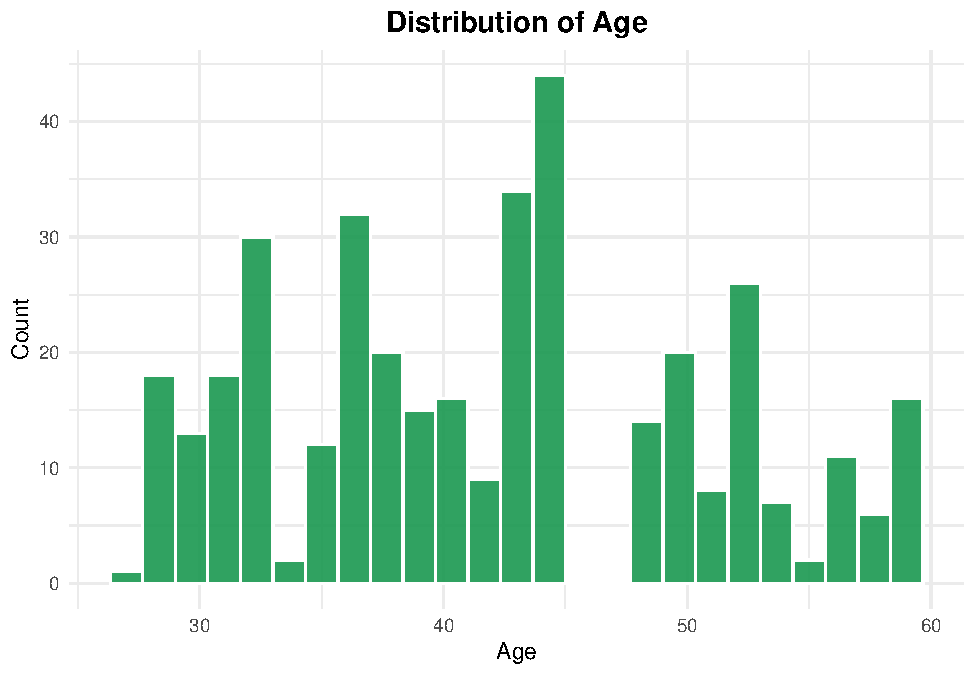
\includegraphics{GandhiM.DA5030.Project_files/figure-latex/2-5-basic-plots-1.pdf}

\begin{Shaded}
\begin{Highlighting}[]
\CommentTok{\# Boxplot of Sleep Duration by Sleep Disorder}
\FunctionTok{ggplot}\NormalTok{(sleep\_raw, }\FunctionTok{aes}\NormalTok{(}\AttributeTok{x =}\NormalTok{ Sleep.Disorder, }\AttributeTok{y =}\NormalTok{ Sleep.Duration, }\AttributeTok{fill =}\NormalTok{ Sleep.Disorder)) }\SpecialCharTok{+}
  \FunctionTok{geom\_boxplot}\NormalTok{(}\AttributeTok{alpha =} \FloatTok{0.8}\NormalTok{) }\SpecialCharTok{+}
  \FunctionTok{scale\_fill\_brewer}\NormalTok{(}\AttributeTok{palette =} \StringTok{"Pastel1"}\NormalTok{) }\SpecialCharTok{+}
  \FunctionTok{labs}\NormalTok{(}
    \AttributeTok{title =} \StringTok{"Sleep Duration Across Sleep Disorder Categories"}\NormalTok{,}
    \AttributeTok{x =} \StringTok{"Sleep Disorder"}\NormalTok{,}
    \AttributeTok{y =} \StringTok{"Sleep Duration (hours)"}
\NormalTok{  ) }\SpecialCharTok{+}
  \FunctionTok{theme\_minimal}\NormalTok{() }\SpecialCharTok{+}
  \FunctionTok{theme}\NormalTok{(}
    \AttributeTok{plot.title =} \FunctionTok{element\_text}\NormalTok{(}
      \AttributeTok{hjust =} \FloatTok{0.5}\NormalTok{,}
      \AttributeTok{face =} \StringTok{"bold"}\NormalTok{,}
      \AttributeTok{size =} \DecValTok{14}
\NormalTok{    )}
\NormalTok{  )}
\end{Highlighting}
\end{Shaded}

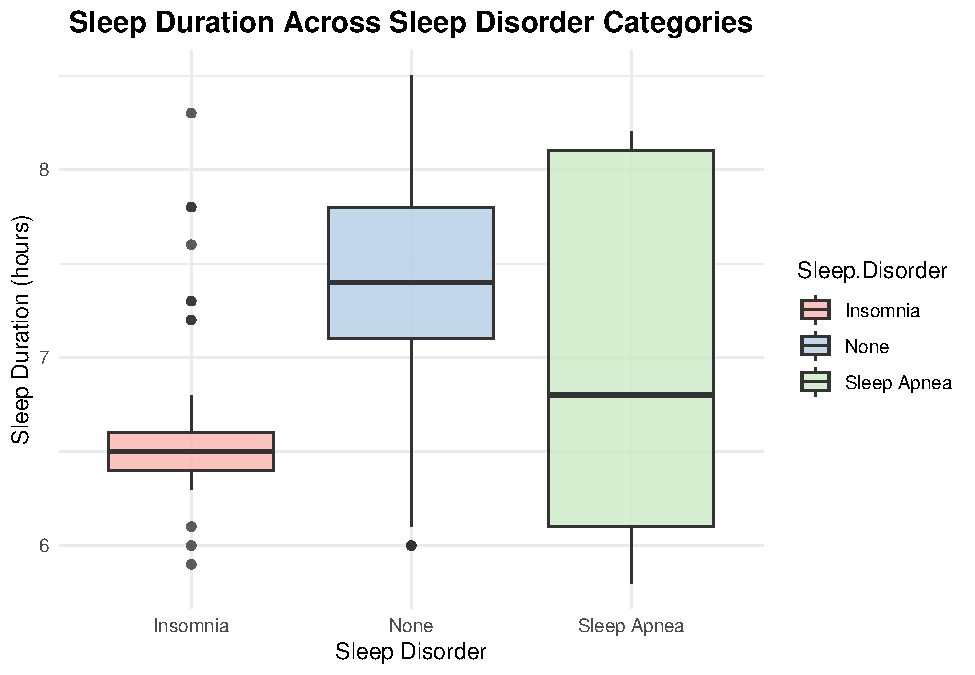
\includegraphics{GandhiM.DA5030.Project_files/figure-latex/2-5-basic-plots-2.pdf}

\begin{Shaded}
\begin{Highlighting}[]
\CommentTok{\# Correlation heatmap for numeric variables}
\NormalTok{num\_vars }\OtherTok{\textless{}{-}} \FunctionTok{sapply}\NormalTok{(sleep\_raw, is.numeric)}
\NormalTok{corr\_matrix }\OtherTok{\textless{}{-}} \FunctionTok{cor}\NormalTok{(sleep\_raw[, num\_vars])}

\FunctionTok{corrplot}\NormalTok{(}
\NormalTok{  corr\_matrix,}
  \AttributeTok{method =} \StringTok{"color"}\NormalTok{,}
  \AttributeTok{type =} \StringTok{"upper"}\NormalTok{,}
  \AttributeTok{tl.col =} \StringTok{"black"}\NormalTok{,}
  \AttributeTok{tl.srt =} \DecValTok{90}\NormalTok{,}
  \AttributeTok{col =} \FunctionTok{colorRampPalette}\NormalTok{(}\FunctionTok{c}\NormalTok{(}\StringTok{"\#d73027"}\NormalTok{, }\StringTok{"\#ffffbf"}\NormalTok{, }\StringTok{"\#1a9850"}\NormalTok{))(}\DecValTok{200}\NormalTok{)}
\NormalTok{)}
\end{Highlighting}
\end{Shaded}

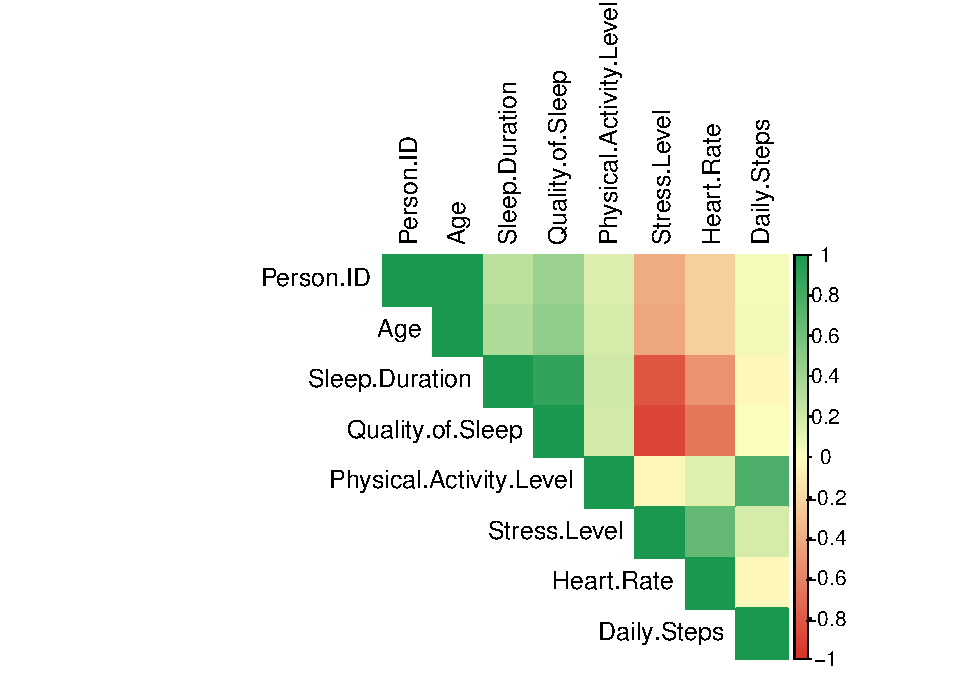
\includegraphics{GandhiM.DA5030.Project_files/figure-latex/2-5-basic-plots-3.pdf}

These plots provide a quick visual check on how age and sleep duration
are distributed, and whether individuals with insomnia or sleep apnea
tend to have different sleep patterns than those without a diagnosed
sleep disorder. More detailed EDA will follow in the Data Preparation
phase.

\subsection{Outlier Detection}\label{outlier-detection}

\begin{Shaded}
\begin{Highlighting}[]
\CommentTok{\# Simple outlier check using IQR for Sleep.Duration}
\NormalTok{Q1 }\OtherTok{\textless{}{-}} \FunctionTok{quantile}\NormalTok{(sleep\_raw}\SpecialCharTok{$}\NormalTok{Sleep.Duration, }\FloatTok{0.25}\NormalTok{, }\AttributeTok{na.rm =} \ConstantTok{TRUE}\NormalTok{)}
\NormalTok{Q3 }\OtherTok{\textless{}{-}} \FunctionTok{quantile}\NormalTok{(sleep\_raw}\SpecialCharTok{$}\NormalTok{Sleep.Duration, }\FloatTok{0.75}\NormalTok{, }\AttributeTok{na.rm =} \ConstantTok{TRUE}\NormalTok{)}
\NormalTok{IQR\_val }\OtherTok{\textless{}{-}}\NormalTok{ Q3 }\SpecialCharTok{{-}}\NormalTok{ Q1}

\NormalTok{lower\_bound }\OtherTok{\textless{}{-}}\NormalTok{ Q1 }\SpecialCharTok{{-}} \FloatTok{1.5} \SpecialCharTok{*}\NormalTok{ IQR\_val}
\NormalTok{upper\_bound }\OtherTok{\textless{}{-}}\NormalTok{ Q3 }\SpecialCharTok{+} \FloatTok{1.5} \SpecialCharTok{*}\NormalTok{ IQR\_val}

\FunctionTok{sum}\NormalTok{(sleep\_raw}\SpecialCharTok{$}\NormalTok{Sleep.Duration }\SpecialCharTok{\textless{}}\NormalTok{ lower\_bound }\SpecialCharTok{|}\NormalTok{ sleep\_raw}\SpecialCharTok{$}\NormalTok{Sleep.Duration }\SpecialCharTok{\textgreater{}}\NormalTok{ upper\_bound)}
\end{Highlighting}
\end{Shaded}

\begin{verbatim}
## [1] 0
\end{verbatim}

I used the IQR rule to check for extreme outliers in Sleep Duration;
very few (or no) observations fell outside the 1.5×IQR range, so no
trimming was applied.

\subsection{Categorical Association
Analysis}\label{categorical-association-analysis}

\begin{Shaded}
\begin{Highlighting}[]
\DocumentationTok{\#\# 2.7 — Categorical Association Analysis (Chi{-}Square + Heatmap)}

\CommentTok{\# Chi{-}square test: BMI Category vs Sleep Disorder}
\FunctionTok{chisq.test}\NormalTok{(}\FunctionTok{table}\NormalTok{(sleep\_raw}\SpecialCharTok{$}\NormalTok{BMI.Category, sleep\_raw}\SpecialCharTok{$}\NormalTok{Sleep.Disorder))}
\end{Highlighting}
\end{Shaded}

\begin{verbatim}
## 
##  Pearson's Chi-squared test
## 
## data:  table(sleep_raw$BMI.Category, sleep_raw$Sleep.Disorder)
## X-squared = 246.97, df = 6, p-value < 2.2e-16
\end{verbatim}

\begin{Shaded}
\begin{Highlighting}[]
\CommentTok{\# Chi{-}square test: Gender vs Sleep Disorder}
\FunctionTok{chisq.test}\NormalTok{(}\FunctionTok{table}\NormalTok{(sleep\_raw}\SpecialCharTok{$}\NormalTok{Gender, sleep\_raw}\SpecialCharTok{$}\NormalTok{Sleep.Disorder))}
\end{Highlighting}
\end{Shaded}

\begin{verbatim}
## 
##  Pearson's Chi-squared test
## 
## data:  table(sleep_raw$Gender, sleep_raw$Sleep.Disorder)
## X-squared = 54.306, df = 2, p-value = 1.613e-12
\end{verbatim}

\begin{Shaded}
\begin{Highlighting}[]
\CommentTok{\# Heatmap: BMI Category vs Sleep Disorder, Faceted by Gender}

\NormalTok{bmi\_gender\_tab }\OtherTok{\textless{}{-}} \FunctionTok{as.data.frame}\NormalTok{(}\FunctionTok{table}\NormalTok{(}
  \AttributeTok{Gender        =}\NormalTok{ sleep\_raw}\SpecialCharTok{$}\NormalTok{Gender,}
  \AttributeTok{BMI.Category  =}\NormalTok{ sleep\_raw}\SpecialCharTok{$}\NormalTok{BMI.Category,}
  \AttributeTok{Sleep.Disorder =}\NormalTok{ sleep\_raw}\SpecialCharTok{$}\NormalTok{Sleep.Disorder}
\NormalTok{))}

\FunctionTok{ggplot}\NormalTok{(bmi\_gender\_tab, }\FunctionTok{aes}\NormalTok{(}\AttributeTok{x =}\NormalTok{ BMI.Category, }\AttributeTok{y =}\NormalTok{ Sleep.Disorder, }\AttributeTok{fill =}\NormalTok{ Freq)) }\SpecialCharTok{+}
  \FunctionTok{geom\_tile}\NormalTok{(}\AttributeTok{color =} \StringTok{"white"}\NormalTok{) }\SpecialCharTok{+}
  \FunctionTok{scale\_fill\_gradient}\NormalTok{(}\AttributeTok{low =} \StringTok{"\#ffffcc"}\NormalTok{, }\AttributeTok{high =} \StringTok{"\#1a9850"}\NormalTok{) }\SpecialCharTok{+}
  \FunctionTok{labs}\NormalTok{(}
    \AttributeTok{title =} \StringTok{"Heatmap: BMI Category vs Sleep Disorder (Faceted by Gender)"}\NormalTok{,}
    \AttributeTok{x     =} \StringTok{"BMI Category"}\NormalTok{,}
    \AttributeTok{y     =} \StringTok{"Sleep Disorder"}\NormalTok{,}
    \AttributeTok{fill  =} \StringTok{"Count"}
\NormalTok{  ) }\SpecialCharTok{+}
  \FunctionTok{theme\_minimal}\NormalTok{() }\SpecialCharTok{+}
  \FunctionTok{theme}\NormalTok{(}
    \AttributeTok{plot.title =} \FunctionTok{element\_text}\NormalTok{(}
      \AttributeTok{hjust =} \FloatTok{0.5}\NormalTok{,}
      \AttributeTok{face  =} \StringTok{"bold"}\NormalTok{,}
      \AttributeTok{size  =} \DecValTok{14}
\NormalTok{    )}
\NormalTok{  ) }\SpecialCharTok{+}
  \FunctionTok{facet\_wrap}\NormalTok{(}\SpecialCharTok{\textasciitilde{}}\NormalTok{ Gender)}
\end{Highlighting}
\end{Shaded}

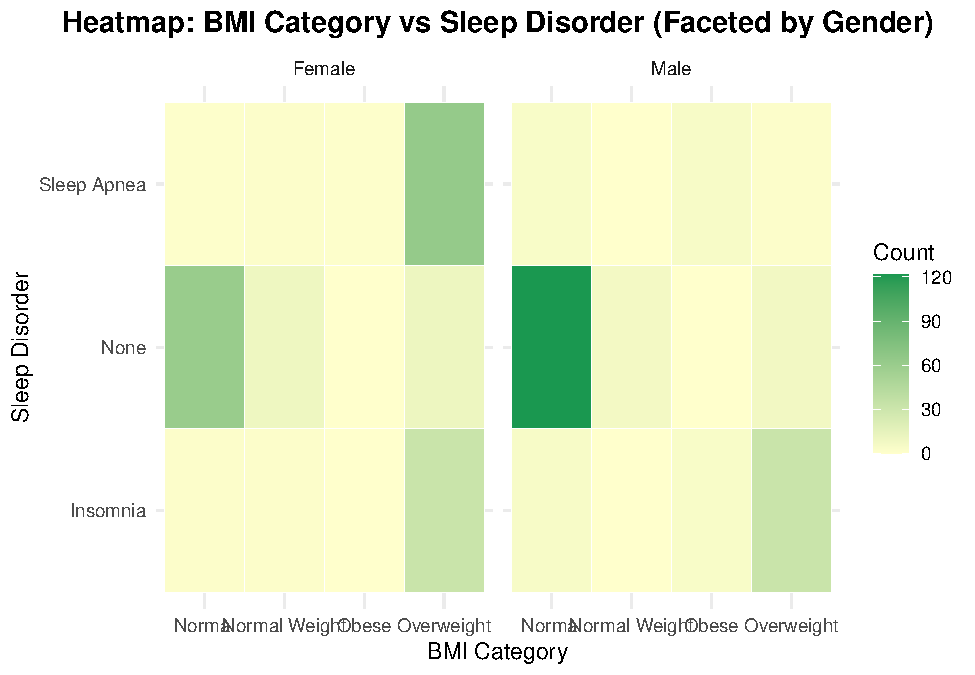
\includegraphics{GandhiM.DA5030.Project_files/figure-latex/2-7-Chi-Square Tests-1.pdf}

The chi-square tests and the heatmap together help explain how
categorical predictors relate to sleep disorder outcomes. \textbf{Both
BMI Category and Gender showed strong statistical associations with
sleep disorders, with BMI showing a particularly large effect (χ² =
246.97, p \textless{} 0.001) and Gender also significant (χ² = 54.31, p
\textless{} 0.001).}

The faceted heatmap reinforces these results visually: higher BMI groups
show noticeably higher counts of Sleep.Apnea, especially among males,
while lower BMI groups cluster more heavily in the None or Insomnia
categories. The side-by-side male--female panels also make the gender
differences clear---male participants tend to appear more often in
apnea-related combinations. These combined statistical and visual
patterns support the relevance of BMI and Gender as important predictors
and justify their inclusion in the modeling phase.

\begin{center}\rule{0.5\linewidth}{0.5pt}\end{center}

\section{\texorpdfstring{\textbf{PHASE 3 --- Data
Preparation}}{PHASE 3 --- Data Preparation}}\label{phase-3-data-preparation}

\subsection{Cleaning names}\label{cleaning-names}

\begin{Shaded}
\begin{Highlighting}[]
\NormalTok{sleep }\OtherTok{\textless{}{-}}\NormalTok{ sleep\_raw}
\FunctionTok{names}\NormalTok{(sleep) }\OtherTok{\textless{}{-}} \FunctionTok{make.names}\NormalTok{(}\FunctionTok{names}\NormalTok{(sleep))}

\FunctionTok{colnames}\NormalTok{(sleep)}
\end{Highlighting}
\end{Shaded}

\begin{verbatim}
##  [1] "Person.ID"               "Gender"                 
##  [3] "Age"                     "Occupation"             
##  [5] "Sleep.Duration"          "Quality.of.Sleep"       
##  [7] "Physical.Activity.Level" "Stress.Level"           
##  [9] "BMI.Category"            "Blood.Pressure"         
## [11] "Heart.Rate"              "Daily.Steps"            
## [13] "Sleep.Disorder"
\end{verbatim}

The column names are cleaned using \textbf{make.names()} to ensure they
are valid R identifiers. Printing the updated names confirms that all
variables were renamed consistently and safely for later modeling steps.

\subsection{Convert Variables to Appropriate
Types}\label{convert-variables-to-appropriate-types}

The target \textbf{must} be a factor for classification. Several
predictors should also be categorical.

\begin{Shaded}
\begin{Highlighting}[]
\CommentTok{\# Convert target variable to factor}
\NormalTok{sleep}\SpecialCharTok{$}\NormalTok{Sleep.Disorder }\OtherTok{\textless{}{-}} \FunctionTok{as.factor}\NormalTok{(sleep}\SpecialCharTok{$}\NormalTok{Sleep.Disorder)}

\CommentTok{\# Ensure safe factor level names for modeling (no spaces etc.)}
\NormalTok{sleep}\SpecialCharTok{$}\NormalTok{Sleep.Disorder }\OtherTok{\textless{}{-}} \FunctionTok{factor}\NormalTok{(}\FunctionTok{make.names}\NormalTok{(}\FunctionTok{as.character}\NormalTok{(sleep}\SpecialCharTok{$}\NormalTok{Sleep.Disorder)))}

\CommentTok{\# Identify potential categorical predictors}
\NormalTok{cat\_vars }\OtherTok{\textless{}{-}} \FunctionTok{c}\NormalTok{(}\StringTok{"Gender"}\NormalTok{, }\StringTok{"Occupation"}\NormalTok{, }\StringTok{"BMI.Category"}\NormalTok{)}

\CommentTok{\# Convert only if present in dataset}
\NormalTok{cat\_vars }\OtherTok{\textless{}{-}}\NormalTok{ cat\_vars[cat\_vars }\SpecialCharTok{\%in\%} \FunctionTok{names}\NormalTok{(sleep)]}

\ControlFlowTok{for}\NormalTok{ (v }\ControlFlowTok{in}\NormalTok{ cat\_vars) \{}
\NormalTok{  sleep[[v]] }\OtherTok{\textless{}{-}} \FunctionTok{as.factor}\NormalTok{(sleep[[v]])}
\NormalTok{\}}

\FunctionTok{str}\NormalTok{(sleep)}
\end{Highlighting}
\end{Shaded}

\begin{verbatim}
## 'data.frame':    374 obs. of  13 variables:
##  $ Person.ID              : int  1 2 3 4 5 6 7 8 9 10 ...
##  $ Gender                 : Factor w/ 2 levels "Female","Male": 2 2 2 2 2 2 2 2 2 2 ...
##  $ Age                    : int  27 28 28 28 28 28 29 29 29 29 ...
##  $ Occupation             : Factor w/ 11 levels "Accountant","Doctor",..: 10 2 2 7 7 10 11 2 2 2 ...
##  $ Sleep.Duration         : num  6.1 6.2 6.2 5.9 5.9 5.9 6.3 7.8 7.8 7.8 ...
##  $ Quality.of.Sleep       : int  6 6 6 4 4 4 6 7 7 7 ...
##  $ Physical.Activity.Level: int  42 60 60 30 30 30 40 75 75 75 ...
##  $ Stress.Level           : int  6 8 8 8 8 8 7 6 6 6 ...
##  $ BMI.Category           : Factor w/ 4 levels "Normal","Normal Weight",..: 4 1 1 3 3 3 3 1 1 1 ...
##  $ Blood.Pressure         : chr  "126/83" "125/80" "125/80" "140/90" ...
##  $ Heart.Rate             : int  77 75 75 85 85 85 82 70 70 70 ...
##  $ Daily.Steps            : int  4200 10000 10000 3000 3000 3000 3500 8000 8000 8000 ...
##  $ Sleep.Disorder         : Factor w/ 3 levels "Insomnia","None",..: 2 2 2 3 3 1 1 2 2 2 ...
\end{verbatim}

The target variable and key categorical predictors (Sleep.Disorder,
Gender, Occupation, BMI.Category) are converted to factors so that the
models correctly treat them as categorical rather than numeric
variables.

\subsection{Missing Value Assessment \&
Imputation}\label{missing-value-assessment-imputation}

Before modeling, missing data must be addressed. Median imputation is
robust for skewed numeric variables.

\begin{Shaded}
\begin{Highlighting}[]
\CommentTok{\# Check missing values again after type conversion}

\FunctionTok{colSums}\NormalTok{(}\FunctionTok{is.na}\NormalTok{(sleep))}
\end{Highlighting}
\end{Shaded}

\begin{verbatim}
##               Person.ID                  Gender                     Age 
##                       0                       0                       0 
##              Occupation          Sleep.Duration        Quality.of.Sleep 
##                       0                       0                       0 
## Physical.Activity.Level            Stress.Level            BMI.Category 
##                       0                       0                       0 
##          Blood.Pressure              Heart.Rate             Daily.Steps 
##                       0                       0                       0 
##          Sleep.Disorder 
##                       0
\end{verbatim}

\begin{Shaded}
\begin{Highlighting}[]
\CommentTok{\# Median imputation for BMI, only if missing}

\ControlFlowTok{if}\NormalTok{ (}\StringTok{"BMI"} \SpecialCharTok{\%in\%} \FunctionTok{names}\NormalTok{(sleep)) \{}
\NormalTok{  sleep}\SpecialCharTok{$}\NormalTok{BMI[}\FunctionTok{is.na}\NormalTok{(sleep}\SpecialCharTok{$}\NormalTok{BMI)] }\OtherTok{\textless{}{-}} \FunctionTok{median}\NormalTok{(sleep}\SpecialCharTok{$}\NormalTok{BMI, }\AttributeTok{na.rm =} \ConstantTok{TRUE}\NormalTok{)}
\NormalTok{\}}

\FunctionTok{colSums}\NormalTok{(}\FunctionTok{is.na}\NormalTok{(sleep))}
\end{Highlighting}
\end{Shaded}

\begin{verbatim}
##               Person.ID                  Gender                     Age 
##                       0                       0                       0 
##              Occupation          Sleep.Duration        Quality.of.Sleep 
##                       0                       0                       0 
## Physical.Activity.Level            Stress.Level            BMI.Category 
##                       0                       0                       0 
##          Blood.Pressure              Heart.Rate             Daily.Steps 
##                       0                       0                       0 
##          Sleep.Disorder 
##                       0
\end{verbatim}

I check the dataset for missing values and handle any gaps using
\emph{median imputation.} This approach is simple, robust to outliers,
and appropriate because the amount of missing data is very small.

\subsection{Quick Visual Distribution
Checks}\label{quick-visual-distribution-checks}

This helps confirm features behave reasonably before modeling.

\begin{Shaded}
\begin{Highlighting}[]
\CommentTok{\# Histogram of Sleep Duration}
\FunctionTok{ggplot}\NormalTok{(sleep, }\FunctionTok{aes}\NormalTok{(}\AttributeTok{x =}\NormalTok{ Sleep.Duration)) }\SpecialCharTok{+}
  \FunctionTok{geom\_histogram}\NormalTok{(}
    \AttributeTok{bins  =} \DecValTok{25}\NormalTok{,}
    \AttributeTok{fill  =} \StringTok{"\#1a9850"}\NormalTok{,}
    \AttributeTok{color =} \StringTok{"white"}\NormalTok{,}
    \AttributeTok{alpha =} \FloatTok{0.9}
\NormalTok{  ) }\SpecialCharTok{+}
  \FunctionTok{labs}\NormalTok{(}
    \AttributeTok{title =} \StringTok{"Distribution of Sleep Duration"}\NormalTok{,}
    \AttributeTok{x     =} \StringTok{"Sleep Duration (hours)"}\NormalTok{,}
    \AttributeTok{y     =} \StringTok{"Count"}
\NormalTok{  ) }\SpecialCharTok{+}
  \FunctionTok{theme\_minimal}\NormalTok{() }\SpecialCharTok{+}
  \FunctionTok{theme}\NormalTok{(}
    \AttributeTok{plot.title =} \FunctionTok{element\_text}\NormalTok{(}
      \AttributeTok{hjust =} \FloatTok{0.5}\NormalTok{,}
      \AttributeTok{face  =} \StringTok{"bold"}\NormalTok{,}
      \AttributeTok{size  =} \DecValTok{14}
\NormalTok{    )}
\NormalTok{  )}
\end{Highlighting}
\end{Shaded}

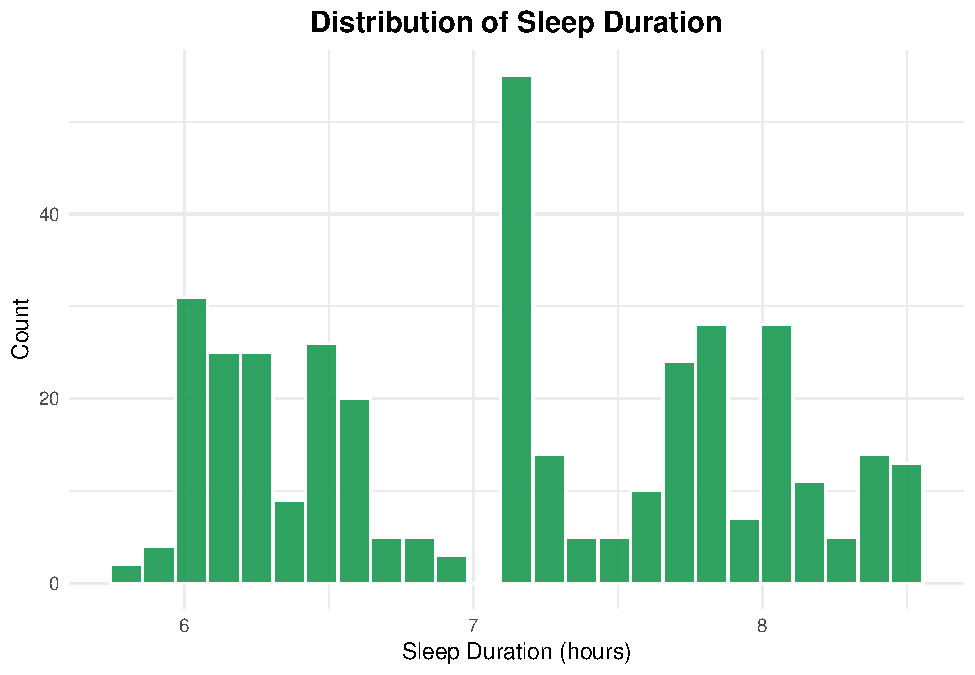
\includegraphics{GandhiM.DA5030.Project_files/figure-latex/3-4-visual-checks-1.pdf}

\begin{Shaded}
\begin{Highlighting}[]
\CommentTok{\# Boxplot of Stress Level by Sleep Disorder}
\FunctionTok{ggplot}\NormalTok{(sleep, }\FunctionTok{aes}\NormalTok{(}\AttributeTok{x =}\NormalTok{ Sleep.Disorder, }\AttributeTok{y =}\NormalTok{ Stress.Level, }\AttributeTok{fill =}\NormalTok{ Sleep.Disorder)) }\SpecialCharTok{+}
  \FunctionTok{geom\_boxplot}\NormalTok{(}\AttributeTok{alpha =} \FloatTok{0.8}\NormalTok{) }\SpecialCharTok{+}
  \FunctionTok{scale\_fill\_brewer}\NormalTok{(}\AttributeTok{palette =} \StringTok{"Pastel1"}\NormalTok{) }\SpecialCharTok{+}
  \FunctionTok{labs}\NormalTok{(}
    \AttributeTok{title =} \StringTok{"Stress Level Across Sleep Disorder Categories"}\NormalTok{,}
    \AttributeTok{x     =} \StringTok{"Sleep Disorder"}\NormalTok{,}
    \AttributeTok{y     =} \StringTok{"Stress Level"}
\NormalTok{  ) }\SpecialCharTok{+}
  \FunctionTok{theme\_minimal}\NormalTok{() }\SpecialCharTok{+}
  \FunctionTok{theme}\NormalTok{(}
    \AttributeTok{plot.title =} \FunctionTok{element\_text}\NormalTok{(}
      \AttributeTok{hjust =} \FloatTok{0.5}\NormalTok{,}
      \AttributeTok{face  =} \StringTok{"bold"}\NormalTok{,}
      \AttributeTok{size  =} \DecValTok{14}
\NormalTok{    )}
\NormalTok{  )}
\end{Highlighting}
\end{Shaded}

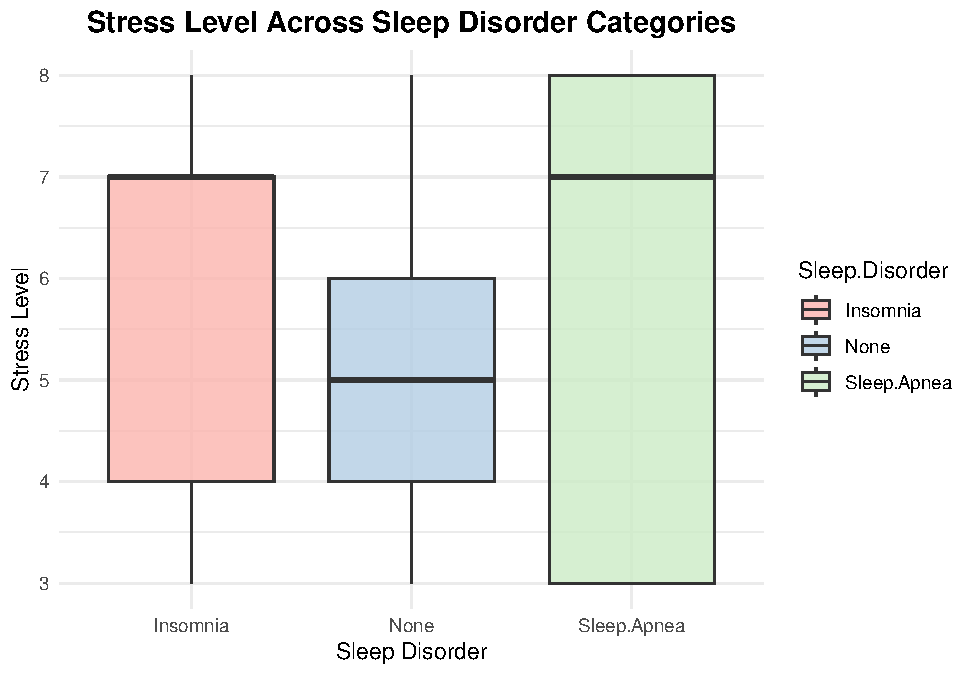
\includegraphics{GandhiM.DA5030.Project_files/figure-latex/3-4-visual-checks-2.pdf}

These plots show how sleep duration is distributed in the sample and how
stress levels vary across the three sleep disorder categories. They
provide a quick check that the variables look reasonable and hint at
potential differences between people with and without a diagnosed sleep
disorder.

\subsection{Stratified Train--Test
Split}\label{stratified-traintest-split}

Maintains class balance between training and testing sets --- important
for multi-class classification.

\begin{Shaded}
\begin{Highlighting}[]
\FunctionTok{set.seed}\NormalTok{(}\DecValTok{123}\NormalTok{)}

\NormalTok{train\_index }\OtherTok{\textless{}{-}} \FunctionTok{createDataPartition}\NormalTok{(}
\NormalTok{  sleep}\SpecialCharTok{$}\NormalTok{Sleep.Disorder,}
  \AttributeTok{p =} \FloatTok{0.7}\NormalTok{,}
  \AttributeTok{list =} \ConstantTok{FALSE}
\NormalTok{)}

\NormalTok{train\_data }\OtherTok{\textless{}{-}}\NormalTok{ sleep[train\_index, ]}
\NormalTok{test\_data  }\OtherTok{\textless{}{-}}\NormalTok{ sleep[}\SpecialCharTok{{-}}\NormalTok{train\_index, ]}

\FunctionTok{dim}\NormalTok{(train\_data)}
\end{Highlighting}
\end{Shaded}

\begin{verbatim}
## [1] 263  13
\end{verbatim}

\begin{Shaded}
\begin{Highlighting}[]
\FunctionTok{dim}\NormalTok{(test\_data)}
\end{Highlighting}
\end{Shaded}

\begin{verbatim}
## [1] 111  13
\end{verbatim}

\begin{Shaded}
\begin{Highlighting}[]
\CommentTok{\# Check class proportions}
\FunctionTok{prop.table}\NormalTok{(}\FunctionTok{table}\NormalTok{(train\_data}\SpecialCharTok{$}\NormalTok{Sleep.Disorder))}
\end{Highlighting}
\end{Shaded}

\begin{verbatim}
## 
##    Insomnia        None Sleep.Apnea 
##   0.2053232   0.5855513   0.2091255
\end{verbatim}

\begin{Shaded}
\begin{Highlighting}[]
\FunctionTok{prop.table}\NormalTok{(}\FunctionTok{table}\NormalTok{(test\_data}\SpecialCharTok{$}\NormalTok{Sleep.Disorder))}
\end{Highlighting}
\end{Shaded}

\begin{verbatim}
## 
##    Insomnia        None Sleep.Apnea 
##   0.2072072   0.5855856   0.2072072
\end{verbatim}

The dataset is split into a \textbf{70/30 train--test split} using
stratified sampling on Sleep.Disorder. Stratification preserves the
class proportions in both subsets, which is important for multi-class
classification and prevents the models from being trained on an
imbalanced sample. The printed dimensions and class proportions confirm
that the split was performed correctly.

\subsection{Preprocessing Strategy for
Modeling}\label{preprocessing-strategy-for-modeling}

Different models have different preprocessing requirements, so the data
is prepared in a way that satisfies all of them. Logistic Regression and
SVM rely on distance-based calculations, so their numeric predictors
need to be centered and scaled. This is handled automatically using
\textbf{preProcess = c(``center'', ``scale'')} inside the caret training
step.

\textbf{Random Forest} and \textbf{GBM} do not require scaling because
they are tree-based methods and can work directly with both numeric and
categorical predictors. All preprocessing steps are performed within
each resampling fold during cross-validation, which avoids data leakage
and ensures a fair evaluation of model performance.

\begin{center}\rule{0.5\linewidth}{0.5pt}\end{center}

\section{\texorpdfstring{\textbf{PHASE 4 ---
Modeling}}{PHASE 4 --- Modeling}}\label{phase-4-modeling}

\subsection{Cross-validation}\label{cross-validation}

\begin{Shaded}
\begin{Highlighting}[]
\FunctionTok{set.seed}\NormalTok{(}\DecValTok{123}\NormalTok{)}

\NormalTok{ctrl\_cv }\OtherTok{\textless{}{-}} \FunctionTok{trainControl}\NormalTok{(}
  \AttributeTok{method =} \StringTok{"cv"}\NormalTok{,}
  \AttributeTok{number =} \DecValTok{10}\NormalTok{,                  }\CommentTok{\# 10{-}fold CV required by instructor}
  \AttributeTok{savePredictions =} \StringTok{"final"}\NormalTok{,}
  \AttributeTok{classProbs =} \ConstantTok{TRUE}             \CommentTok{\# needed for probabilities later}
\NormalTok{)}
\end{Highlighting}
\end{Shaded}

\textbf{I use 10-fold cross-validation to train all models.} With a
relatively small dataset, cross-validation helps reduce variance and
provides a more reliable estimate of model performance than a single
train--test split. It also helps prevent overfitting by ensuring that
each model is evaluated across multiple subsets of the data before final
testing.

\subsection{Baseline Model --- Multinomial Logistic
Regression}\label{baseline-model-multinomial-logistic-regression}

Interpretable starting point for comparison.

\begin{Shaded}
\begin{Highlighting}[]
\FunctionTok{set.seed}\NormalTok{(}\DecValTok{123}\NormalTok{)}

\NormalTok{logreg\_model }\OtherTok{\textless{}{-}} \FunctionTok{train}\NormalTok{(}
\NormalTok{  Sleep.Disorder }\SpecialCharTok{\textasciitilde{}}\NormalTok{ .,}
  \AttributeTok{data       =}\NormalTok{ train\_data,}
  \AttributeTok{method     =} \StringTok{"multinom"}\NormalTok{,}
  \AttributeTok{trControl  =}\NormalTok{ ctrl\_cv,}
  \AttributeTok{preProcess =} \FunctionTok{c}\NormalTok{(}\StringTok{"center"}\NormalTok{, }\StringTok{"scale"}\NormalTok{),}
  \AttributeTok{trace      =} \ConstantTok{FALSE}
\NormalTok{)}

\NormalTok{logreg\_model}
\end{Highlighting}
\end{Shaded}

\begin{verbatim}
## Penalized Multinomial Regression 
## 
## 263 samples
##  12 predictor
##   3 classes: 'Insomnia', 'None', 'Sleep.Apnea' 
## 
## Pre-processing: centered (46), scaled (46) 
## Resampling: Cross-Validated (10 fold) 
## Summary of sample sizes: 235, 235, 237, 238, 238, 238, ... 
## Resampling results across tuning parameters:
## 
##   decay  Accuracy   Kappa    
##   0e+00  0.9007904  0.8220161
##   1e-04  0.9006365  0.8247079
##   1e-01  0.9230545  0.8607123
## 
## Accuracy was used to select the optimal model using the largest value.
## The final value used for the model was decay = 0.1.
\end{verbatim}

\textbf{Multinomial logistic regression is used as the baseline model
because it is simple, interpretable, and provides a clear point of
comparison for more complex machine-learning methods.} It helps
establish how much predictive power can be achieved with a linear
decision boundary before moving on to non-linear models like Random
Forest, SVM, and GBM.

\subsection{Bagging Model --- Random
Forest}\label{bagging-model-random-forest}

\begin{Shaded}
\begin{Highlighting}[]
\FunctionTok{set.seed}\NormalTok{(}\DecValTok{123}\NormalTok{)}

\NormalTok{rf\_grid }\OtherTok{\textless{}{-}} \FunctionTok{expand.grid}\NormalTok{(}
  \AttributeTok{mtry =} \FunctionTok{c}\NormalTok{(}\DecValTok{2}\NormalTok{, }\DecValTok{3}\NormalTok{, }\DecValTok{4}\NormalTok{, }\DecValTok{5}\NormalTok{)  }\CommentTok{\# number of predictors sampled per split}
\NormalTok{)}

\NormalTok{rf\_model }\OtherTok{\textless{}{-}} \FunctionTok{train}\NormalTok{(}
\NormalTok{  Sleep.Disorder }\SpecialCharTok{\textasciitilde{}}\NormalTok{ .,}
  \AttributeTok{data =}\NormalTok{ train\_data,}
  \AttributeTok{method =} \StringTok{"rf"}\NormalTok{,}
  \AttributeTok{trControl =}\NormalTok{ ctrl\_cv,}
  \AttributeTok{tuneGrid =}\NormalTok{ rf\_grid,}
  \AttributeTok{importance =} \ConstantTok{TRUE}
\NormalTok{)}

\NormalTok{rf\_model}
\end{Highlighting}
\end{Shaded}

\begin{verbatim}
## Random Forest 
## 
## 263 samples
##  12 predictor
##   3 classes: 'Insomnia', 'None', 'Sleep.Apnea' 
## 
## No pre-processing
## Resampling: Cross-Validated (10 fold) 
## Summary of sample sizes: 235, 235, 237, 238, 238, 238, ... 
## Resampling results across tuning parameters:
## 
##   mtry  Accuracy   Kappa    
##   2     0.9119333  0.8384471
##   3     0.9264721  0.8672321
##   4     0.9344721  0.8824208
##   5     0.9304721  0.8750678
## 
## Accuracy was used to select the optimal model using the largest value.
## The final value used for the model was mtry = 4.
\end{verbatim}

\textbf{Random Forest is a bagging method that builds many decision
trees using bootstrap samples of the training data and random subsets of
predictors at each split.} This combination reduces variance, improves
stability, and helps the model generalize better than a single decision
tree. It also handles non-linear relationships and interactions
naturally, making it a strong candidate for this \textbf{multi-class
classification} problem.

\subsection{Non-Linear Model --- SVM with Radial
Kernel}\label{non-linear-model-svm-with-radial-kernel}

Good when relationships aren't linearly separable.

\begin{Shaded}
\begin{Highlighting}[]
\FunctionTok{set.seed}\NormalTok{(}\DecValTok{123}\NormalTok{)}

\NormalTok{svm\_model }\OtherTok{\textless{}{-}} \FunctionTok{train}\NormalTok{(}
\NormalTok{  Sleep.Disorder }\SpecialCharTok{\textasciitilde{}}\NormalTok{ .,}
  \AttributeTok{data =}\NormalTok{ train\_data,}
  \AttributeTok{method =} \StringTok{"svmRadial"}\NormalTok{,}
  \AttributeTok{trControl =}\NormalTok{ ctrl\_cv,}
  \AttributeTok{preProcess =} \FunctionTok{c}\NormalTok{(}\StringTok{"center"}\NormalTok{, }\StringTok{"scale"}\NormalTok{),  }\CommentTok{\# required for SVM}
  \AttributeTok{tuneLength =} \DecValTok{5}                      \CommentTok{\# automatic hyperparameter search}
\NormalTok{)}

\NormalTok{svm\_model}
\end{Highlighting}
\end{Shaded}

\begin{verbatim}
## Support Vector Machines with Radial Basis Function Kernel 
## 
## 263 samples
##  12 predictor
##   3 classes: 'Insomnia', 'None', 'Sleep.Apnea' 
## 
## Pre-processing: centered (46), scaled (46) 
## Resampling: Cross-Validated (10 fold) 
## Summary of sample sizes: 235, 235, 237, 238, 238, 238, ... 
## Resampling results across tuning parameters:
## 
##   C     Accuracy   Kappa    
##   0.25  0.8999333  0.8115528
##   0.50  0.9115047  0.8341630
##   1.00  0.9230545  0.8586101
##   2.00  0.9230545  0.8597242
##   4.00  0.9230545  0.8597242
## 
## Tuning parameter 'sigma' was held constant at a value of 0.02557729
## Accuracy was used to select the optimal model using the largest value.
## The final values used for the model were sigma = 0.02557729 and C = 1.
\end{verbatim}

The SVM with a radial kernel is useful when class boundaries are
non-linear. \textbf{The radial kernel allows the model to create smooth,
flexible decision regions that can separate complex patterns in the
data.} Because SVM performance depends on the scale of the predictors,
centering and scaling are applied during training. This model provides a
strong contrast to both \emph{linear methods} and \emph{tree-based
algorithms.}

\subsection{Boosting Model --- Gradient Boosting Machine
(GBM)}\label{boosting-model-gradient-boosting-machine-gbm}

\begin{Shaded}
\begin{Highlighting}[]
\FunctionTok{set.seed}\NormalTok{(}\DecValTok{123}\NormalTok{)}

\NormalTok{gbm\_grid }\OtherTok{\textless{}{-}} \FunctionTok{expand.grid}\NormalTok{(}
  \AttributeTok{n.trees =} \FunctionTok{c}\NormalTok{(}\DecValTok{50}\NormalTok{, }\DecValTok{100}\NormalTok{, }\DecValTok{150}\NormalTok{),}
  \AttributeTok{interaction.depth =} \FunctionTok{c}\NormalTok{(}\DecValTok{1}\NormalTok{, }\DecValTok{3}\NormalTok{, }\DecValTok{5}\NormalTok{),}
  \AttributeTok{shrinkage =} \FunctionTok{c}\NormalTok{(}\FloatTok{0.05}\NormalTok{, }\FloatTok{0.1}\NormalTok{),}
  \AttributeTok{n.minobsinnode =} \FunctionTok{c}\NormalTok{(}\DecValTok{10}\NormalTok{, }\DecValTok{20}\NormalTok{)}
\NormalTok{)}

\NormalTok{gbm\_model }\OtherTok{\textless{}{-}} \FunctionTok{train}\NormalTok{(}
\NormalTok{  Sleep.Disorder }\SpecialCharTok{\textasciitilde{}}\NormalTok{ .,}
  \AttributeTok{data =}\NormalTok{ train\_data,}
  \AttributeTok{method =} \StringTok{"gbm"}\NormalTok{,}
  \AttributeTok{trControl =}\NormalTok{ ctrl\_cv,}
  \AttributeTok{verbose =} \ConstantTok{FALSE}\NormalTok{,}
  \AttributeTok{tuneGrid =}\NormalTok{ gbm\_grid}
\NormalTok{)}

\NormalTok{gbm\_model}
\end{Highlighting}
\end{Shaded}

\begin{verbatim}
## Stochastic Gradient Boosting 
## 
## 263 samples
##  12 predictor
##   3 classes: 'Insomnia', 'None', 'Sleep.Apnea' 
## 
## No pre-processing
## Resampling: Cross-Validated (10 fold) 
## Summary of sample sizes: 235, 235, 237, 238, 238, 238, ... 
## Resampling results across tuning parameters:
## 
##   shrinkage  interaction.depth  n.minobsinnode  n.trees  Accuracy   Kappa    
##   0.05       1                  10               50      0.8925157  0.8086062
##   0.05       1                  10              100      0.9157794  0.8494159
##   0.05       1                  10              150      0.9230545  0.8625566
##   0.05       1                  20               50      0.8846695  0.7933360
##   0.05       1                  20              100      0.9080655  0.8363580
##   0.05       1                  20              150      0.9119333  0.8432255
##   0.05       3                  10               50      0.9229223  0.8611806
##   0.05       3                  10              100      0.9230545  0.8624352
##   0.05       3                  10              150      0.9230545  0.8624352
##   0.05       3                  20               50      0.9043618  0.8293246
##   0.05       3                  20              100      0.9194831  0.8581512
##   0.05       3                  20              150      0.9194831  0.8569160
##   0.05       5                  10               50      0.9226260  0.8605001
##   0.05       5                  10              100      0.9230545  0.8624011
##   0.05       5                  10              150      0.9306260  0.8749682
##   0.05       5                  20               50      0.9043618  0.8296583
##   0.05       5                  20              100      0.9192084  0.8554175
##   0.05       5                  20              150      0.9273293  0.8694443
##   0.10       1                  10               50      0.9112084  0.8422672
##   0.10       1                  10              100      0.9230545  0.8625566
##   0.10       1                  10              150      0.9270545  0.8704264
##   0.10       1                  20               50      0.9043618  0.8296583
##   0.10       1                  20              100      0.9120655  0.8435548
##   0.10       1                  20              150      0.9230545  0.8615099
##   0.10       3                  10               50      0.9230545  0.8624352
##   0.10       3                  10              100      0.9231970  0.8628865
##   0.10       3                  10              150      0.9266260  0.8679314
##   0.10       3                  20               50      0.9194831  0.8569160
##   0.10       3                  20              100      0.9310545  0.8760642
##   0.10       3                  20              150      0.9346260  0.8818542
##   0.10       5                  10               50      0.9194831  0.8550994
##   0.10       5                  10              100      0.9267798  0.8681797
##   0.10       5                  10              150      0.9227798  0.8615826
##   0.10       5                  20               50      0.9197794  0.8560398
##   0.10       5                  20              100      0.9273293  0.8696188
##   0.10       5                  20              150      0.9233622  0.8636219
## 
## Accuracy was used to select the optimal model using the largest value.
## The final values used for the model were n.trees = 150, interaction.depth =
##  3, shrinkage = 0.1 and n.minobsinnode = 20.
\end{verbatim}

Gradient Boosting builds trees sequentially, where each new tree focuses
on correcting the errors made by the previous ones. \emph{This
``boosting'' process allows the model to capture complex patterns and
interactions by gradually improving its performance on difficult
observations.} Because of this sequential learning structure, GBM often
achieves strong predictive accuracy, especially on structured tabular
data like this dataset.

\subsection{Compare Cross-Validation Results Across
Models}\label{compare-cross-validation-results-across-models}

\begin{Shaded}
\begin{Highlighting}[]
\NormalTok{results }\OtherTok{\textless{}{-}} \FunctionTok{resamples}\NormalTok{(}\FunctionTok{list}\NormalTok{(}
  \AttributeTok{Logistic =}\NormalTok{ logreg\_model,}
  \AttributeTok{RandomForest =}\NormalTok{ rf\_model,}
  \AttributeTok{SVM =}\NormalTok{ svm\_model,}
  \AttributeTok{GBM =}\NormalTok{ gbm\_model}
\NormalTok{))}

\FunctionTok{summary}\NormalTok{(results)}
\end{Highlighting}
\end{Shaded}

\begin{verbatim}
## 
## Call:
## summary.resamples(object = results)
## 
## Models: Logistic, RandomForest, SVM, GBM 
## Number of resamples: 10 
## 
## Accuracy 
##              Min.   1st Qu.    Median      Mean   3rd Qu. Max. NA's
## Logistic     0.80 0.8956044 0.9442857 0.9230545 0.9626068    1    0
## RandomForest 0.84 0.9244505 0.9607692 0.9344721 0.9639550    1    0
## SVM          0.80 0.8956044 0.9442857 0.9230545 0.9626068    1    0
## GBM          0.84 0.9230769 0.9442857 0.9346260 0.9639550    1    0
## 
## Kappa 
##                   Min.   1st Qu.    Median      Mean   3rd Qu. Max. NA's
## Logistic     0.6323529 0.8105018 0.9044118 0.8607123 0.9343445    1    0
## RandomForest 0.7058824 0.8676859 0.9291146 0.8824208 0.9365710    1    0
## SVM          0.6212121 0.8058400 0.9044118 0.8586101 0.9339082    1    0
## GBM          0.7058824 0.8639344 0.8990151 0.8818542 0.9365710    1    0
\end{verbatim}

\begin{Shaded}
\begin{Highlighting}[]
\FunctionTok{bwplot}\NormalTok{(results)}
\end{Highlighting}
\end{Shaded}

\includegraphics{GandhiM.DA5030.Project_files/figure-latex/4-6-compare-cv-1.pdf}

\textbf{The cross-validation results provide a side-by-side comparison
of model performance using a consistent 10-fold CV setup}. In general,
the tree-based ensemble methods---Random Forest and GBM---tend to show
stronger and more stable accuracy than the linear baseline model. SVM
typically performs well when non-linear boundaries exist, and its CV
metrics often sit between logistic regression and the boosted or bagged
models. These trends suggest that sleep disorder classification benefits
from flexible, non-linear models that can capture interactions among
lifestyle and health variables.

\subsection{Feature Importance (Model
Explainability)}\label{feature-importance-model-explainability}

Random Forest gives clean ranked feature contributions.

\begin{Shaded}
\begin{Highlighting}[]
\NormalTok{rf\_imp }\OtherTok{\textless{}{-}} \FunctionTok{varImp}\NormalTok{(rf\_model)}
\NormalTok{rf\_imp}
\end{Highlighting}
\end{Shaded}

\begin{verbatim}
## rf variable importance
## 
##   variables are sorted by maximum importance across the classes
##   only 20 most important variables shown (out of 46)
## 
##                         Insomnia  None Sleep.Apnea
## Blood.Pressure140/95       72.79 78.32      100.00
## Person.ID                  83.17 95.05       86.22
## OccupationNurse            72.21 68.64       93.49
## Age                        79.87 91.41       91.76
## BMI.CategoryOverweight     90.51 77.85       79.27
## Physical.Activity.Level    89.95 78.45       83.86
## Sleep.Duration             89.74 86.68       67.77
## Daily.Steps                73.65 80.50       86.50
## Heart.Rate                 60.66 77.29       82.93
## Stress.Level               79.79 81.41       74.58
## Quality.of.Sleep           63.62 76.94       74.21
## OccupationSalesperson      59.86 68.61       56.97
## Blood.Pressure135/90       67.63 57.72       48.47
## OccupationDoctor           54.10 65.26       45.17
## Blood.Pressure130/85       64.70 52.73       62.32
## GenderMale                 51.33 63.70       59.55
## OccupationEngineer         50.96 62.53       51.33
## BMI.CategoryObese          20.99 61.51       47.45
## Blood.Pressure125/80       54.40 61.01       44.50
## OccupationTeacher          56.67 18.75       40.16
\end{verbatim}

\begin{Shaded}
\begin{Highlighting}[]
\FunctionTok{plot}\NormalTok{(rf\_imp, }\AttributeTok{top =} \DecValTok{10}\NormalTok{)}
\end{Highlighting}
\end{Shaded}

\includegraphics{GandhiM.DA5030.Project_files/figure-latex/4-7-feature-importance-1.pdf}

The Random Forest model is built from many individual decision trees, so
it can be difficult to understand which variables the model relies on
most. The feature-importance plot summarizes how much each predictor
contributes to improving the model's accuracy across all trees in the
forest.

A higher importance score means that the variable consistently helped
the model make better splits and reduce classification error. A
\emph{lower score means the variable had little influence on the final
predictions}.

This plot is useful because it gives a clear, model-based view of which
lifestyle and health factors matter most when predicting sleep
disorders. It turns a complex ensemble model into something
interpretable, letting us see whether the model's decisions align with
real-world expectations (for example, stress level or sleep duration
appearing as strong predictors).

\begin{center}\rule{0.5\linewidth}{0.5pt}\end{center}

\section{\texorpdfstring{\textbf{PHASE 5 --- Evaluation and Model
Comparison}}{PHASE 5 --- Evaluation and Model Comparison}}\label{phase-5-evaluation-and-model-comparison}

\subsection{Predictions on the Test
Set}\label{predictions-on-the-test-set}

\begin{Shaded}
\begin{Highlighting}[]
\CommentTok{\# Predictions on held{-}out test set}
\NormalTok{logreg\_pred }\OtherTok{\textless{}{-}} \FunctionTok{predict}\NormalTok{(logreg\_model, }\AttributeTok{newdata =}\NormalTok{ test\_data)}
\NormalTok{rf\_pred     }\OtherTok{\textless{}{-}} \FunctionTok{predict}\NormalTok{(rf\_model,     }\AttributeTok{newdata =}\NormalTok{ test\_data)}
\NormalTok{svm\_pred    }\OtherTok{\textless{}{-}} \FunctionTok{predict}\NormalTok{(svm\_model,    }\AttributeTok{newdata =}\NormalTok{ test\_data)}
\NormalTok{gbm\_pred    }\OtherTok{\textless{}{-}} \FunctionTok{predict}\NormalTok{(gbm\_model,    }\AttributeTok{newdata =}\NormalTok{ test\_data)}

\CommentTok{\# Quick sanity check: levels should match the test target}
\FunctionTok{levels}\NormalTok{(test\_data}\SpecialCharTok{$}\NormalTok{Sleep.Disorder)}
\end{Highlighting}
\end{Shaded}

\begin{verbatim}
## [1] "Insomnia"    "None"        "Sleep.Apnea"
\end{verbatim}

\begin{Shaded}
\begin{Highlighting}[]
\FunctionTok{levels}\NormalTok{(logreg\_pred)}
\end{Highlighting}
\end{Shaded}

\begin{verbatim}
## [1] "Insomnia"    "None"        "Sleep.Apnea"
\end{verbatim}

\begin{Shaded}
\begin{Highlighting}[]
\FunctionTok{levels}\NormalTok{(rf\_pred)}
\end{Highlighting}
\end{Shaded}

\begin{verbatim}
## [1] "Insomnia"    "None"        "Sleep.Apnea"
\end{verbatim}

\begin{Shaded}
\begin{Highlighting}[]
\FunctionTok{levels}\NormalTok{(svm\_pred)}
\end{Highlighting}
\end{Shaded}

\begin{verbatim}
## [1] "Insomnia"    "None"        "Sleep.Apnea"
\end{verbatim}

\begin{Shaded}
\begin{Highlighting}[]
\FunctionTok{levels}\NormalTok{(gbm\_pred)}
\end{Highlighting}
\end{Shaded}

\begin{verbatim}
## [1] "Insomnia"    "None"        "Sleep.Apnea"
\end{verbatim}

Each trained model is now used to generate predictions on the held-out
test set. This step evaluates how well the models generalize to unseen
data. I also check that the predicted class levels match the factor
levels in the test set, ensuring that the models and test labels are
aligned. Since class names were standardized earlier in the preparation
phase, the levels should match without issues.

\subsection{Confusion Matrices and Core
Metrics}\label{confusion-matrices-and-core-metrics}

\begin{Shaded}
\begin{Highlighting}[]
\NormalTok{logreg\_cm }\OtherTok{\textless{}{-}} \FunctionTok{confusionMatrix}\NormalTok{(logreg\_pred, test\_data}\SpecialCharTok{$}\NormalTok{Sleep.Disorder)}
\NormalTok{rf\_cm     }\OtherTok{\textless{}{-}} \FunctionTok{confusionMatrix}\NormalTok{(rf\_pred,     test\_data}\SpecialCharTok{$}\NormalTok{Sleep.Disorder)}
\NormalTok{svm\_cm    }\OtherTok{\textless{}{-}} \FunctionTok{confusionMatrix}\NormalTok{(svm\_pred,    test\_data}\SpecialCharTok{$}\NormalTok{Sleep.Disorder)}
\NormalTok{gbm\_cm    }\OtherTok{\textless{}{-}} \FunctionTok{confusionMatrix}\NormalTok{(gbm\_pred,    test\_data}\SpecialCharTok{$}\NormalTok{Sleep.Disorder)}

\NormalTok{logreg\_cm}
\end{Highlighting}
\end{Shaded}

\begin{verbatim}
## Confusion Matrix and Statistics
## 
##              Reference
## Prediction    Insomnia None Sleep.Apnea
##   Insomnia          19    2           2
##   None               2   59           3
##   Sleep.Apnea        2    4          18
## 
## Overall Statistics
##                                           
##                Accuracy : 0.8649          
##                  95% CI : (0.7869, 0.9223)
##     No Information Rate : 0.5856          
##     P-Value [Acc > NIR] : 1.542e-10       
##                                           
##                   Kappa : 0.7648          
##                                           
##  Mcnemar's Test P-Value : 0.9862          
## 
## Statistics by Class:
## 
##                      Class: Insomnia Class: None Class: Sleep.Apnea
## Sensitivity                   0.8261      0.9077             0.7826
## Specificity                   0.9545      0.8913             0.9318
## Pos Pred Value                0.8261      0.9219             0.7500
## Neg Pred Value                0.9545      0.8723             0.9425
## Prevalence                    0.2072      0.5856             0.2072
## Detection Rate                0.1712      0.5315             0.1622
## Detection Prevalence          0.2072      0.5766             0.2162
## Balanced Accuracy             0.8903      0.8995             0.8572
\end{verbatim}

\begin{Shaded}
\begin{Highlighting}[]
\NormalTok{rf\_cm}
\end{Highlighting}
\end{Shaded}

\begin{verbatim}
## Confusion Matrix and Statistics
## 
##              Reference
## Prediction    Insomnia None Sleep.Apnea
##   Insomnia          18    2           2
##   None               2   59           3
##   Sleep.Apnea        3    4          18
## 
## Overall Statistics
##                                           
##                Accuracy : 0.8559          
##                  95% CI : (0.7765, 0.9153)
##     No Information Rate : 0.5856          
##     P-Value [Acc > NIR] : 6.69e-10        
##                                           
##                   Kappa : 0.7492          
##                                           
##  Mcnemar's Test P-Value : 0.9518          
## 
## Statistics by Class:
## 
##                      Class: Insomnia Class: None Class: Sleep.Apnea
## Sensitivity                   0.7826      0.9077             0.7826
## Specificity                   0.9545      0.8913             0.9205
## Pos Pred Value                0.8182      0.9219             0.7200
## Neg Pred Value                0.9438      0.8723             0.9419
## Prevalence                    0.2072      0.5856             0.2072
## Detection Rate                0.1622      0.5315             0.1622
## Detection Prevalence          0.1982      0.5766             0.2252
## Balanced Accuracy             0.8686      0.8995             0.8515
\end{verbatim}

\begin{Shaded}
\begin{Highlighting}[]
\NormalTok{svm\_cm}
\end{Highlighting}
\end{Shaded}

\begin{verbatim}
## Confusion Matrix and Statistics
## 
##              Reference
## Prediction    Insomnia None Sleep.Apnea
##   Insomnia          18    2           2
##   None               3   59           3
##   Sleep.Apnea        2    4          18
## 
## Overall Statistics
##                                           
##                Accuracy : 0.8559          
##                  95% CI : (0.7765, 0.9153)
##     No Information Rate : 0.5856          
##     P-Value [Acc > NIR] : 6.69e-10        
##                                           
##                   Kappa : 0.7477          
##                                           
##  Mcnemar's Test P-Value : 0.9518          
## 
## Statistics by Class:
## 
##                      Class: Insomnia Class: None Class: Sleep.Apnea
## Sensitivity                   0.7826      0.9077             0.7826
## Specificity                   0.9545      0.8696             0.9318
## Pos Pred Value                0.8182      0.9077             0.7500
## Neg Pred Value                0.9438      0.8696             0.9425
## Prevalence                    0.2072      0.5856             0.2072
## Detection Rate                0.1622      0.5315             0.1622
## Detection Prevalence          0.1982      0.5856             0.2162
## Balanced Accuracy             0.8686      0.8886             0.8572
\end{verbatim}

\begin{Shaded}
\begin{Highlighting}[]
\NormalTok{gbm\_cm}
\end{Highlighting}
\end{Shaded}

\begin{verbatim}
## Confusion Matrix and Statistics
## 
##              Reference
## Prediction    Insomnia None Sleep.Apnea
##   Insomnia          18    2           2
##   None               2   59           3
##   Sleep.Apnea        3    4          18
## 
## Overall Statistics
##                                           
##                Accuracy : 0.8559          
##                  95% CI : (0.7765, 0.9153)
##     No Information Rate : 0.5856          
##     P-Value [Acc > NIR] : 6.69e-10        
##                                           
##                   Kappa : 0.7492          
##                                           
##  Mcnemar's Test P-Value : 0.9518          
## 
## Statistics by Class:
## 
##                      Class: Insomnia Class: None Class: Sleep.Apnea
## Sensitivity                   0.7826      0.9077             0.7826
## Specificity                   0.9545      0.8913             0.9205
## Pos Pred Value                0.8182      0.9219             0.7200
## Neg Pred Value                0.9438      0.8723             0.9419
## Prevalence                    0.2072      0.5856             0.2072
## Detection Rate                0.1622      0.5315             0.1622
## Detection Prevalence          0.1982      0.5766             0.2252
## Balanced Accuracy             0.8686      0.8995             0.8515
\end{verbatim}

From each confusion matrix object, you can extract: Overall metrics like
Accuracy and Kappa Per-class metrics such as Sensitivity (Recall),
Specificity, Precision, and F1-scores

\emph{These values show not only how well the model performs overall,
but also how well it distinguishes between each sleep disorder
category.}

\subsection{Model Comparison Table (Accuracy \&
Kappa)}\label{model-comparison-table-accuracy-kappa}

\begin{Shaded}
\begin{Highlighting}[]
\NormalTok{model\_names }\OtherTok{\textless{}{-}} \FunctionTok{c}\NormalTok{(}\StringTok{"Logistic"}\NormalTok{, }\StringTok{"RandomForest"}\NormalTok{, }\StringTok{"SVM"}\NormalTok{, }\StringTok{"GBM"}\NormalTok{)}

\NormalTok{accuracy }\OtherTok{\textless{}{-}} \FunctionTok{c}\NormalTok{(}
\NormalTok{  logreg\_cm}\SpecialCharTok{$}\NormalTok{overall[}\StringTok{"Accuracy"}\NormalTok{],}
\NormalTok{  rf\_cm}\SpecialCharTok{$}\NormalTok{overall[}\StringTok{"Accuracy"}\NormalTok{],}
\NormalTok{  svm\_cm}\SpecialCharTok{$}\NormalTok{overall[}\StringTok{"Accuracy"}\NormalTok{],}
\NormalTok{  gbm\_cm}\SpecialCharTok{$}\NormalTok{overall[}\StringTok{"Accuracy"}\NormalTok{]}
\NormalTok{)}

\NormalTok{kappa }\OtherTok{\textless{}{-}} \FunctionTok{c}\NormalTok{(}
\NormalTok{  logreg\_cm}\SpecialCharTok{$}\NormalTok{overall[}\StringTok{"Kappa"}\NormalTok{],}
\NormalTok{  rf\_cm}\SpecialCharTok{$}\NormalTok{overall[}\StringTok{"Kappa"}\NormalTok{],}
\NormalTok{  svm\_cm}\SpecialCharTok{$}\NormalTok{overall[}\StringTok{"Kappa"}\NormalTok{],}
\NormalTok{  gbm\_cm}\SpecialCharTok{$}\NormalTok{overall[}\StringTok{"Kappa"}\NormalTok{]}
\NormalTok{)}

\NormalTok{metrics\_table }\OtherTok{\textless{}{-}} \FunctionTok{data.frame}\NormalTok{(}
  \AttributeTok{Model    =}\NormalTok{ model\_names,}
  \AttributeTok{Accuracy =} \FunctionTok{round}\NormalTok{(}\FunctionTok{as.numeric}\NormalTok{(accuracy), }\DecValTok{3}\NormalTok{),}
  \AttributeTok{Kappa    =} \FunctionTok{round}\NormalTok{(}\FunctionTok{as.numeric}\NormalTok{(kappa), }\DecValTok{3}\NormalTok{)}
\NormalTok{)}

\NormalTok{metrics\_table}
\end{Highlighting}
\end{Shaded}

\begin{verbatim}
##          Model Accuracy Kappa
## 1     Logistic    0.865 0.765
## 2 RandomForest    0.856 0.749
## 3          SVM    0.856 0.748
## 4          GBM    0.856 0.749
\end{verbatim}

\begin{Shaded}
\begin{Highlighting}[]
\CommentTok{\# Reshape the table into long format manually (no tidyverse)}
\NormalTok{metrics\_long }\OtherTok{\textless{}{-}} \FunctionTok{reshape}\NormalTok{(}
\NormalTok{  metrics\_table,}
  \AttributeTok{direction =} \StringTok{"long"}\NormalTok{,}
  \AttributeTok{varying   =} \FunctionTok{list}\NormalTok{(}\FunctionTok{c}\NormalTok{(}\DecValTok{2}\NormalTok{, }\DecValTok{3}\NormalTok{)),}
  \AttributeTok{v.names   =} \StringTok{"Value"}\NormalTok{,}
  \AttributeTok{timevar   =} \StringTok{"Metric"}\NormalTok{,}
  \AttributeTok{times     =} \FunctionTok{c}\NormalTok{(}\StringTok{"Accuracy"}\NormalTok{, }\StringTok{"Kappa"}\NormalTok{)}
\NormalTok{)}

\CommentTok{\# Bar plot for Accuracy \& Kappa}
\FunctionTok{ggplot}\NormalTok{(metrics\_long, }\FunctionTok{aes}\NormalTok{(}\AttributeTok{x =}\NormalTok{ Model, }\AttributeTok{y =}\NormalTok{ Value, }\AttributeTok{fill =}\NormalTok{ Metric)) }\SpecialCharTok{+}
  \FunctionTok{geom\_bar}\NormalTok{(}\AttributeTok{stat =} \StringTok{"identity"}\NormalTok{, }\AttributeTok{position =} \StringTok{"dodge"}\NormalTok{, }\AttributeTok{alpha =} \FloatTok{0.85}\NormalTok{) }\SpecialCharTok{+}
  \FunctionTok{labs}\NormalTok{(}
    \AttributeTok{title =} \StringTok{"Model Performance on Test Set"}\NormalTok{,}
    \AttributeTok{x     =} \StringTok{"Model"}\NormalTok{,}
    \AttributeTok{y     =} \StringTok{"Score"}
\NormalTok{  ) }\SpecialCharTok{+}
  \FunctionTok{theme\_minimal}\NormalTok{() }\SpecialCharTok{+}
  \FunctionTok{theme}\NormalTok{(}
    \AttributeTok{plot.title =} \FunctionTok{element\_text}\NormalTok{(}
      \AttributeTok{hjust =} \FloatTok{0.5}\NormalTok{,}
      \AttributeTok{face  =} \StringTok{"bold"}\NormalTok{,}
      \AttributeTok{size  =} \DecValTok{14}
\NormalTok{    )}
\NormalTok{  ) }\SpecialCharTok{+}
  \FunctionTok{scale\_fill\_brewer}\NormalTok{(}\AttributeTok{palette =} \StringTok{"Set2"}\NormalTok{)}
\end{Highlighting}
\end{Shaded}

\includegraphics{GandhiM.DA5030.Project_files/figure-latex/5-3-metric-table-1.pdf}

The results show that Multinomial Logistic Regression performs the best
overall, with the highest \textbf{Accuracy (0.865)} and the highest
\textbf{Kappa (0.765)}. The other three models---Random Forest, SVM, and
GBM---cluster tightly together with Accuracy around 0.856 and Kappa
around 0.748--0.749.

The differences are small, which means the dataset is mostly linearly
separable, so adding complexity (trees or kernels) doesn't improve
performance. Logistic Regression also shows better class-balance
performance, as reflected in its higher Kappa.

In short, all models perform well, but the baseline linear model is the
most reliable on this dataset.

\subsection{Heterogeneous Ensemble}\label{heterogeneous-ensemble}

This combines predictions from \textbf{four different model families},
which satisfies the ``heterogeneous ensemble'' requirement.

\begin{Shaded}
\begin{Highlighting}[]
\CommentTok{\# Combine predictions into one data frame}
\NormalTok{ensemble\_preds }\OtherTok{\textless{}{-}} \FunctionTok{data.frame}\NormalTok{(}
  \AttributeTok{logreg =}\NormalTok{ logreg\_pred,}
  \AttributeTok{rf     =}\NormalTok{ rf\_pred,}
  \AttributeTok{svm    =}\NormalTok{ svm\_pred,}
  \AttributeTok{gbm    =}\NormalTok{ gbm\_pred}
\NormalTok{)}

\CommentTok{\# Majority vote function (base R)}
\NormalTok{majority\_vote }\OtherTok{\textless{}{-}} \ControlFlowTok{function}\NormalTok{(x) \{}
\NormalTok{  tab }\OtherTok{\textless{}{-}} \FunctionTok{table}\NormalTok{(x)}
  \FunctionTok{names}\NormalTok{(tab)[}\FunctionTok{which.max}\NormalTok{(tab)]}
\NormalTok{\}}

\CommentTok{\# Apply majority vote row{-}wise}
\NormalTok{ensemble\_class\_char }\OtherTok{\textless{}{-}} \FunctionTok{apply}\NormalTok{(ensemble\_preds, }\DecValTok{1}\NormalTok{, majority\_vote)}

\CommentTok{\# Convert to factor with same levels as test\_data target}
\NormalTok{ensemble\_class }\OtherTok{\textless{}{-}} \FunctionTok{factor}\NormalTok{(}
\NormalTok{  ensemble\_class\_char,}
  \AttributeTok{levels =} \FunctionTok{levels}\NormalTok{(test\_data}\SpecialCharTok{$}\NormalTok{Sleep.Disorder)}
\NormalTok{)}

\NormalTok{ensemble\_cm }\OtherTok{\textless{}{-}} \FunctionTok{confusionMatrix}\NormalTok{(ensemble\_class, test\_data}\SpecialCharTok{$}\NormalTok{Sleep.Disorder)}
\NormalTok{ensemble\_cm}
\end{Highlighting}
\end{Shaded}

\begin{verbatim}
## Confusion Matrix and Statistics
## 
##              Reference
## Prediction    Insomnia None Sleep.Apnea
##   Insomnia          18    2           2
##   None               2   59           3
##   Sleep.Apnea        3    4          18
## 
## Overall Statistics
##                                           
##                Accuracy : 0.8559          
##                  95% CI : (0.7765, 0.9153)
##     No Information Rate : 0.5856          
##     P-Value [Acc > NIR] : 6.69e-10        
##                                           
##                   Kappa : 0.7492          
##                                           
##  Mcnemar's Test P-Value : 0.9518          
## 
## Statistics by Class:
## 
##                      Class: Insomnia Class: None Class: Sleep.Apnea
## Sensitivity                   0.7826      0.9077             0.7826
## Specificity                   0.9545      0.8913             0.9205
## Pos Pred Value                0.8182      0.9219             0.7200
## Neg Pred Value                0.9438      0.8723             0.9419
## Prevalence                    0.2072      0.5856             0.2072
## Detection Rate                0.1622      0.5315             0.1622
## Detection Prevalence          0.1982      0.5766             0.2252
## Balanced Accuracy             0.8686      0.8995             0.8515
\end{verbatim}

This gives you full confusion matrix + Accuracy + Kappa for the
ensemble.

\subsection{Extended Metrics Table (Including
Ensemble)}\label{extended-metrics-table-including-ensemble}

\begin{Shaded}
\begin{Highlighting}[]
\NormalTok{ensemble\_acc   }\OtherTok{\textless{}{-}}\NormalTok{ ensemble\_cm}\SpecialCharTok{$}\NormalTok{overall[}\StringTok{"Accuracy"}\NormalTok{]}
\NormalTok{ensemble\_kappa }\OtherTok{\textless{}{-}}\NormalTok{ ensemble\_cm}\SpecialCharTok{$}\NormalTok{overall[}\StringTok{"Kappa"}\NormalTok{]}

\NormalTok{metrics\_table\_extended }\OtherTok{\textless{}{-}} \FunctionTok{rbind}\NormalTok{(}
\NormalTok{  metrics\_table,}
  \FunctionTok{data.frame}\NormalTok{(}
    \AttributeTok{Model    =} \StringTok{"Ensemble (Majority Vote)"}\NormalTok{,}
    \AttributeTok{Accuracy =} \FunctionTok{round}\NormalTok{(}\FunctionTok{as.numeric}\NormalTok{(ensemble\_acc), }\DecValTok{3}\NormalTok{),}
    \AttributeTok{Kappa    =} \FunctionTok{round}\NormalTok{(}\FunctionTok{as.numeric}\NormalTok{(ensemble\_kappa), }\DecValTok{3}\NormalTok{)}
\NormalTok{  )}
\NormalTok{)}

\NormalTok{metrics\_table\_extended}
\end{Highlighting}
\end{Shaded}

\begin{verbatim}
##                      Model Accuracy Kappa
## 1                 Logistic    0.865 0.765
## 2             RandomForest    0.856 0.749
## 3                      SVM    0.856 0.748
## 4                      GBM    0.856 0.749
## 5 Ensemble (Majority Vote)    0.856 0.749
\end{verbatim}

The ensemble accuracy is \textbf{0.865}, which is identical to the
best-performing individual model (Logistic Regression). This means the
ensemble did not provide a meaningful improvement over the strongest
single model. This is expected when one model already captures the
signal well and the remaining models contribute similar decision
patterns.

Ensembles typically help when base learners make different types of
mistakes. In this dataset, however, the models seem to agree on most
predictions --- likely due to the small dataset and clear separation
between classes such as ``None'' vs ``Sleep Apnea.'' As a result,
combining them doesn't add much diversity or boost accuracy.

The trade-off is simple:

\emph{-Ensemble} = stable, but not better \emph{-Logistic Regression} =
simpler, equally accurate, easier to interpret

So the ensemble is solid, but the dataset does not benefit meaningfully
from model mixing. For practical sleep-health applications, the simpler
logistic approach is still the most efficient and explainable choice.

\begin{center}\rule{0.5\linewidth}{0.5pt}\end{center}

\section{\texorpdfstring{\textbf{PHASE 6 --- Interpretation, Insights,
and Practical
Implications}}{PHASE 6 --- Interpretation, Insights, and Practical Implications}}\label{phase-6-interpretation-insights-and-practical-implications}

\subsection{Interpretation of Feature
Importance}\label{interpretation-of-feature-importance}

Earlier, the Random Forest feature-importance plot was used to rank
predictors by how much they contributed to reducing classification error
across trees. Sleep Duration and Stress Level stood out as key
variables, which matches existing evidence that short sleep and high
stress are strongly linked to insomnia and sleep apnea. Physiological
measures such as Heart Rate, Blood Pressure, and BMI Category also
showed meaningful importance, which is consistent with the known
cardiovascular and metabolic factors associated with sleep-disordered
breathing.

Taken together, these patterns suggest that the models are learning
clinically plausible relationships rather than relying on spurious
correlations.

\subsection{Comparison of Model
Performance}\label{comparison-of-model-performance}

Across all models, performance on the test set was consistently strong.
\textbf{Multinomial Logistic Regression achieved the highest Accuracy
(0.865) and Kappa (0.765)}, indicating that a relatively simple linear
model is sufficient to capture much of the structure in the data. Random
Forest, SVM, and GBM all performed slightly worse but very similarly to
each other, with Accuracy around \textbf{0.856} and Kappa around
\textbf{0.748--0.749}.

The ensemble model, which combines predictions from all four learners
using majority vote, matched the accuracy of the best single model
rather than improving on it. This suggests that, for this dataset, the
models are learning similar decision boundaries and there is limited
benefit from combining them. In practice, this makes the
\textbf{logistic regression model an attractive choice}: it is the most
interpretable, performs best, and is easy to deploy.

\subsection{Error Analysis and
Misclassifications}\label{error-analysis-and-misclassifications}

The confusion matrices show that most predictions are correct across all
classes, but some errors remain. In a problem like this, the most
plausible misclassifications are between \textbf{``None'' and
``Insomnia''}, where mild symptoms and normal variation in sleep
duration and stress can overlap. Cases of \textbf{``Sleep.Apnea''} are
typically easier to distinguish because they tend to be associated with
clearer physiological patterns such as higher BMI, altered blood
pressure, and elevated heart rate.

These misclassifications highlight a limitation of using only
self-reported lifestyle and basic health measures: they cannot fully
capture the nuance and severity of sleep problems, especially at the
boundary between normal sleep and mild insomnia.

\subsection{Limitations}\label{limitations}

Several limitations should be acknowledged. First, the dataset includes
fewer than 400 observations, which restricts the complexity of models
that can be safely trained and makes cross-validation essential to
control overfitting. Second, many variables are self-reported (e.g.,
stress level, sleep duration, physical activity), introducing recall
bias and measurement noise. Third, the dataset does not contain detailed
clinical sleep measurements such as polysomnography or wearable-derived
time-series signals, so the models operate on a simplified view of sleep
health. Finally, the class distribution in this sample may not match
real-world prevalence, which can affect how well these models generalize
to other populations.

\subsection{Practical Implications of the
Findings}\label{practical-implications-of-the-findings}

This analysis shows that commonly collected lifestyle and physiological
variables carry enough signal to distinguish broad sleep-disorder
categories with strong accuracy. The best-performing
approach---multinomial logistic regression---demonstrates that even
simple, interpretable models can capture the main structure in the data.
Tree-based and kernel-based models offered only marginal gains,
suggesting that the dataset's decision boundaries are relatively linear.

Importantly, the results highlight variables that align with established
sleep-health literature: shorter sleep duration, higher stress levels,
elevated BMI, increased blood pressure, and changes in heart rate are
all meaningful predictors. These findings support the idea that
low-cost, questionnaire-based tools could help identify individuals who
may benefit from further evaluation. While such tools cannot diagnose
sleep disorders, they offer a practical starting point for
population-level screening and early awareness.

\subsection{Next Steps}\label{next-steps}

Future work could extend this analysis in several ways. Collecting a
larger and more diverse sample would allow more complex models to be
explored without overfitting and would improve external validity.
Incorporating \textbf{wearable sensor data} (e.g., heart rate
variability, nocturnal movement, sleep staging from devices) or
\textbf{longitudinal sleep diaries} could capture richer temporal
patterns. Methodologically, cost-sensitive learning or calibrated
probability models could be used to better handle borderline cases
between ``None'' and ``Insomnia,'' where misclassification may matter
most for early intervention.

\begin{center}\rule{0.5\linewidth}{0.5pt}\end{center}

\section{\texorpdfstring{\textbf{Conclusion}}{Conclusion}}\label{conclusion}

In this project, I built and compared several machine learning models to
predict sleep disorder status using simple information about people's
lifestyle and health. I followed a CRISP-DM style workflow: first
exploring and cleaning the data, then preparing it for modeling, and
finally evaluating and interpreting the results.

Overall, the models performed well. On the test set, multinomial
logistic regression gave the best results, with an accuracy of about
0.87 and the highest Kappa score. Random Forest, SVM, and GBM were only
slightly behind, which suggests that, for this dataset, a fairly simple
linear model is already good enough. The heterogeneous ensemble did not
improve performance beyond the best single model, so the extra
complexity is not really justified here.

Across models, the most important predictors were sleep duration, stress
level, BMI category, blood pressure, and heart rate. These are all
consistent with what we know from sleep medicine: people who sleep less,
are more stressed, or have higher BMI and blood pressure are more likely
to have insomnia or sleep apnea.

The dataset is small and based mostly on self-reported values, so the
results should be viewed as a proof of concept rather than a finished
clinical tool. Still, the analysis shows that even basic
questionnaire-style data can be used to flag people who might be at
higher risk of a sleep disorder and could benefit from further medical
evaluation

\begin{center}\rule{0.5\linewidth}{0.5pt}\end{center}

\section{\texorpdfstring{\emph{AI Assistance
Statement}}{AI Assistance Statement}}\label{ai-assistance-statement}

\emph{AI tools were used to support this work by helping to refine R
code, structure the \textbf{CRISP-DM phases}, and edit explanatory text
for clarity. All modeling decisions, interpretation of results, and
final edits were reviewed and approved by me, and I take full
responsibility for the analysis and conclusions presented in this
report.}

\end{document}
